
\begin{figure}
  \caption{The cost curves for the real-world datasets.}
  \label{fig:cost-curves-real-world-datasets}
  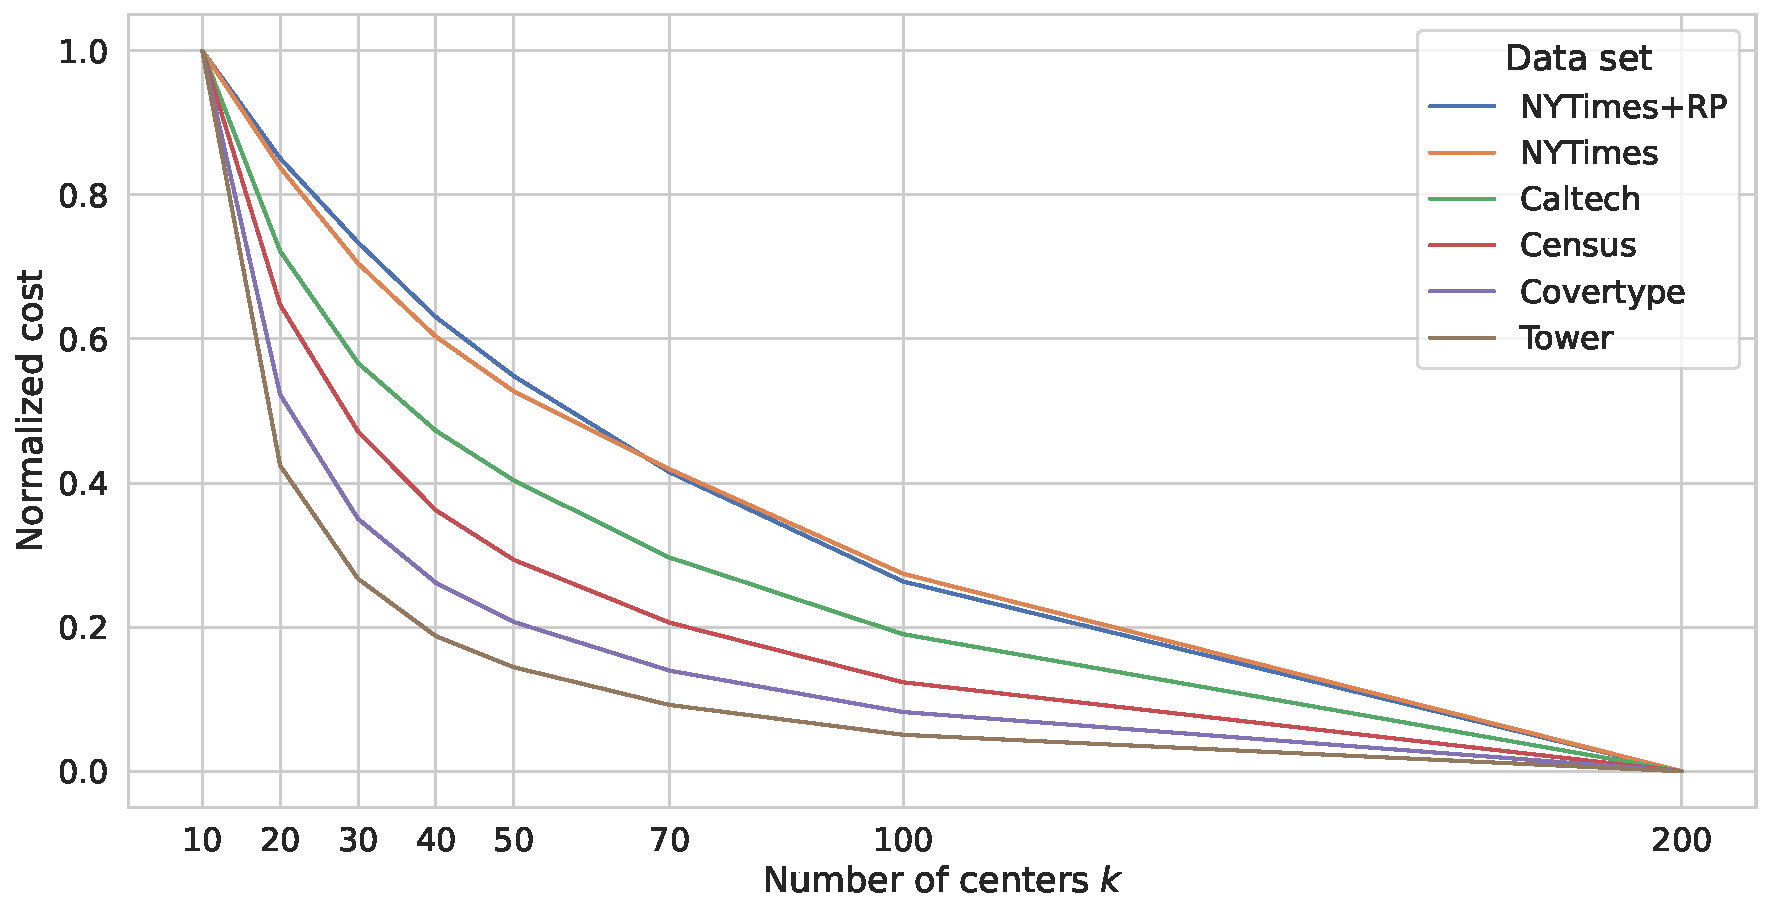
\includegraphics[width=1\linewidth]{figures/cost-curves-real-world-datasets.pdf}
\end{figure}


\begin{figure}
  \caption{The cost curves for the benchmark.}
  \label{fig:cost-curves-benchmark}
  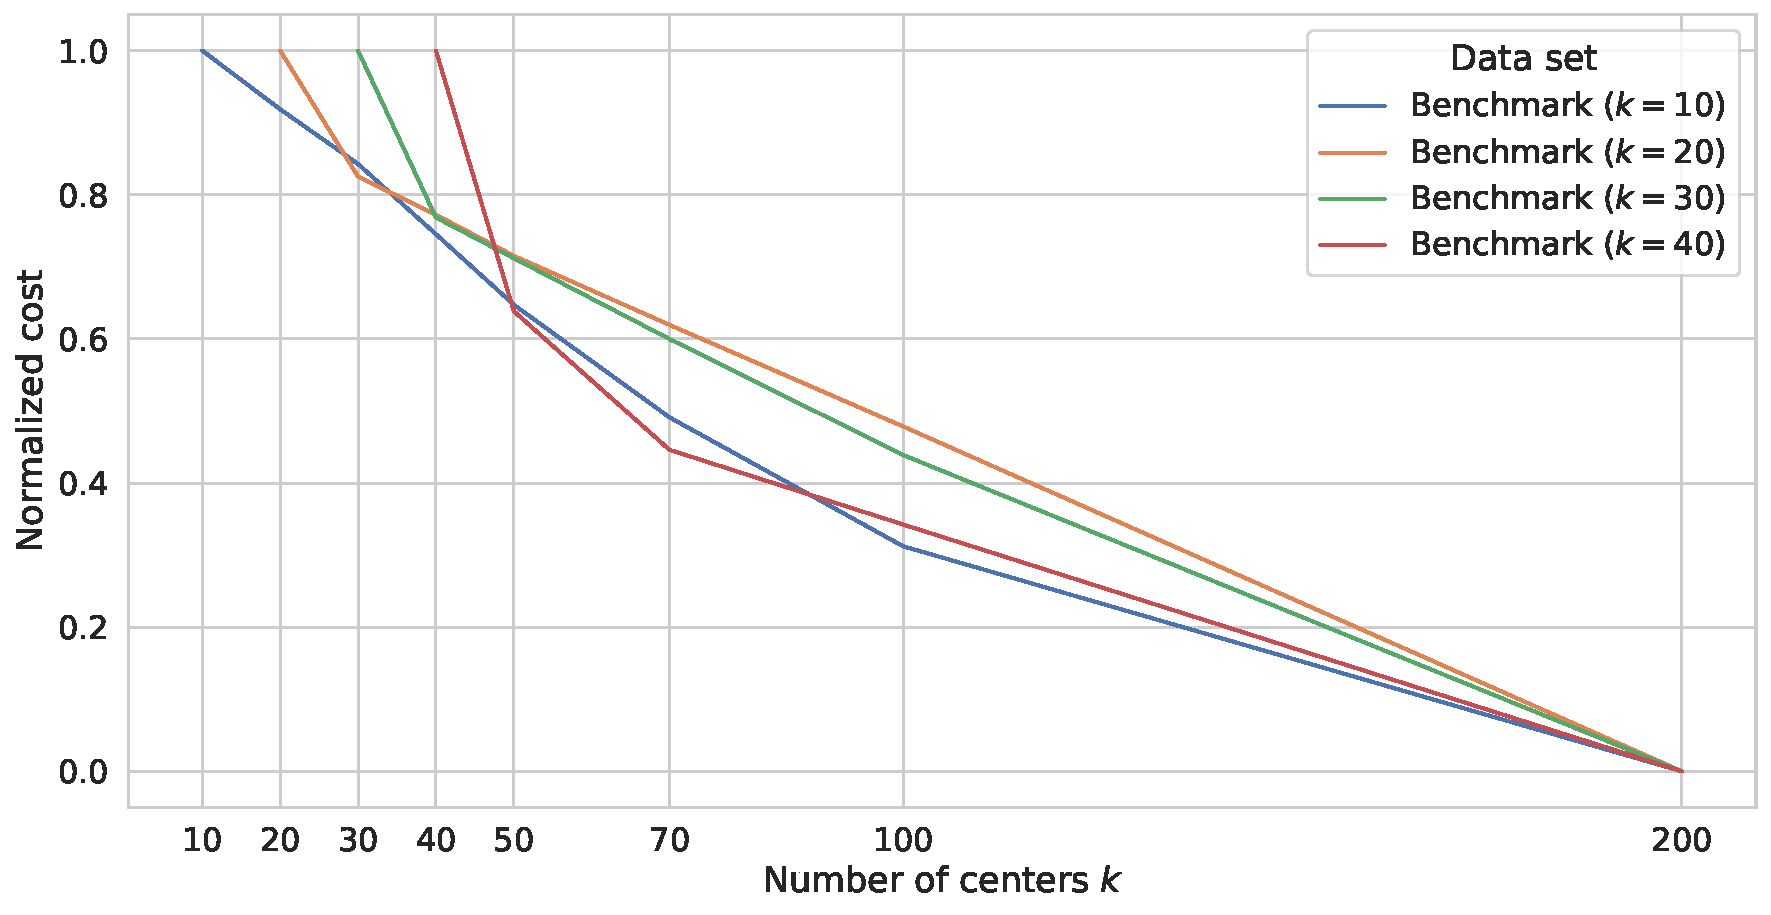
\includegraphics[width=1\linewidth]{figures/cost-curves-benchmark.pdf}
\end{figure}


\section{Experiments} \label{sec:experiments}
In this section, we present a new procedure for evaluating $k$-means coresets. 
We begin our exposition by motivating why there is a need for a new evaluation procedure. Then we describe the proposed procedure, the data sets used for the empirical evaluation and the experimental setup. Finally, we detail the outcome of the experiments and our observations on the results.


\subsection{Motivation for Introducing New Evaluation Procedure}
Previous works evaluated coreset algorithms by comparing the cost of applying a coreset algorithm followed by an optimization procedure. The drawback of this type of evaluation is that it mixes up the two separate tasks of coreset construction and optimization. A coreset algorithm may yield a good clustering (with small cost) yet fail to produce a high quality coreset (with small distortion).
As such, the performance of a coreset algorithm cannot be fully determined by the outcome of the optimization procedure. 

To accurately evaluate a $k$-means coreset in isolation, one would need to come up with a solution i.e., a $k$-center clustering that results in the maximal distortion. In \cref{sec:coreset-evaluation-hard}, we showed that finding such a solution is co-NP hard. How about using a random solution? The issue is that it is not clear how to define a distribution of meaningful solutions from which to sample from. Moreover, a randomly drawn solution, which does not exploit the behavior of a coreset construction, is less likely to yield a worst-case solution in terms of high distortion. A better approach of finding meaningful solutions is to use $k$-means++ as it can uncover cluster structures in the data. Running multiple iterations of $k$-means++ allows us to pick a solution with a high distortion.





As a complement to the evaluation procedure above on real-world data sets, we also proposed a synthetic benchmark for two main reasons. 
% 
First, the benchmark allows us to quickly find a bad solution because both good and bad clusterings are known a priori. This is difficult on real-world data sets.
% 
Second, it is easier to make a fair comparison of different coreset constructions because the benchmark is known to generate hard instances for any coreset algorithm. This is not always the case on real-world data sets.
For example, it is not uncommon for the $k$-means cost to drop significantly for larger values of $k$ in real-world datasets.
~\cref{fig:cost-curves-real-world-datasets} illustrate this behavior for several real-world datasets. The more the curve bends, the less of a difference there is between computing a coreset and a clustering with low cost. In this case, a coreset algorithm adding more centers to the coreset will seem to be performing well when evaluating it based on the outcome of the optimization. However, in the benchmark dataset, there is no way of reducing the cost without capturing the right subclusters within the benchmark instance. This means that the cost does not decrease markedly beyond a certain value of $k$ even if more centers are added as depicted in~\cref{fig:cost-curves-benchmark}.
% In this work, we nevertheless study real-world data sets to determine whether the difference between coresets and optimization can be observed in these data sets.




\subsection{Evaluation Procedure}
For estimating the quality of the coresets produced by various coreset algorithms, we evaluated the algorithms on both real-world data sets and the proposed benchmark. 

On each real-world data set $A$, we first computed a coreset $\Omega$ and then ran $k$-means++ on $\Omega$ to find a set of $k$ centers $\calS$. The $k$-means++ algorithm was repeated 5 times in order to pick the set of centers with the largest distortion. Recall that distortion of a given solution $\calS$ is defined as:
\begin{align*}
    \max\left(
      \frac{\cost_A(\calS)}{\cost_{\Omega}(\calS)},
      \frac{\cost_{\Omega}(\calS)}{\cost_A(\calS)}
    \right)
\end{align*}
For the benchmark, we computed the distortion following the evaluation procedure described in~\cref{sec:benchmark}. Due to the stochastic nature of the algorithms, this experiment was repeated $10$ times. We aggregated the reported distortions by taking the maximum over all $10$ evaluations. In addition, we also preprocessed the data using the dimension reduction techniques described in Section~\ref{sec:algorithms}.


% We now present the empirical evaluation of these coresets.
% We ran two kinds of experiments. On real-world data sets, we merely computed a coreset $\Omega$, followed by running $k$-means++ on $\Omega$. 
% The $k$-means++ algorithm was repeated 5 times, each yielding a solution $\calS_i$, and as the best lower bound on the distortion we used the largest ratio $\max_i\left(\max\left(\frac{\cost_A(\calS_i)}{\cost_{\Omega}(\calS_i)},\frac{\cost_{\Omega}(\calS_i)}{\cost_A(\calS_i)}\right)\right)$.
% For the benchmark, we used the evaluation as proposed in Section~\ref{sec:benchmark}. In addition, we also determined the distortion via simply running the $k$-means++ algorithm. 

% Except for BICO, which is deterministic, this experiment was repeated for each coreset algorithm $10$ times. \omar{Experiments were repeated 10 times including BICO. Although vanilla BICO is deterministic, we used BICO with heuristic speed optimizations which are stochastic.} We aggregated the reported distortions by taking the maximum over all $10$ evaluations. In addition, we also preprocessed the data using the dimension reduction techniques described in Section~\ref{sec:algorithms}.


\subsection{Data sets}
We conducted experiments on 5 real-world data sets. 
The sizes of these data sets are summarized in ~\cref{tab:real-world-datasets-overview}. In addition, we evaluated the behavior of the coreset algorithms using four instances of the proposed benchmark. These instances were generated to match approximately the sizes of the real-world data sets. The chosen parameters values and the corresponding instance sizes are shown in ~\cref{tab:benchmark-instances-overview}. 
% We generated a set of instances with no scaling i.e., $\beta=1.0$ (referred to as \textit{Benchmark-1.0}) and with maximum scaling; $\beta = 2.0$ (\textit{Benchmark-2.0}).
We now provide a brief description of each of the real-world data sets.

The \textit{Census}\footnote{\url{https://archive.ics.uci.edu/ml/datasets/US+Census+Data+(1990)}} dataset is a small subset of the Public Use Microdata Samples from 1990 US census. It consists of demographic information encoded as 68 categorical attributes of 2,458,285 individuals. 

\textit{Covertype}\footnote{\url{https://archive.ics.uci.edu/ml/datasets/covertype}} is comprised of cartographic descriptions and forest cover type of four wilderness areas in the Roosevelt National Forest of Northern Colorado in the US. It consists of 581,012 records, 54 cartographic variables and one class variable. Although \textit{Covertype} was originally made for classification tasks, it is often used for clustering tasks by removing the class variable~\cite{AckermannMRSLS12}.

The data set with the fewest number of dimensions is \textit{Tower}\footnote{\url{http://homepages.uni-paderborn.de/frahling/coremeans.html}}. This data set consists of 4,915,200 rows and 3 features as it is a 2,560 by 1,920 picture of a tower on a hill where each pixel is represented by a RGB color value. 

% We used the datasets \textit{Census}, \textit{Covertype} and \textit{Tower} as these are often used to evaluate the performance of coreset algorithms. 

% To include larger datasets in evaluation, we used \textit{Caltech} and \textit{NYTimes}. 

Inspired by~\cite{FGSSS13}, \textit{Caltech} was created by computing SIFT features from the images in the Caltech101\footnote{\url{http://www.vision.caltech.edu/Image_Datasets/Caltech101/}} image database. This database contains pictures of objects partitioned into 101 categories. Disregarding the categories, we concatenated the 128-dimensional SIFT vectors from each image into one large data matrix. 

% \textit{NYTimes}\footnote{\url{https://archive.ics.uci.edu/ml/datasets/bag+of+words}} dataset in our experiments as the number of dimensions is very large.
\textit{NYTimes}\footnote{\url{https://archive.ics.uci.edu/ml/datasets/bag+of+words}} is a dataset composed of the bag-of-words (BOW) representations of 300,000 news articles from The New York Times. The vocabulary size of the text collection is 102,660. Due to the BOW encoding, \textit{NYTimes} has a very large number of dimensions and is highly sparse. To make processing feasible, we reduced the number of dimensions to 100 using terminal embeddings.

\subsection{Preprocessing \& Experimental Setup}
To understand how denoising effects the quality of the outputted coresets, we applied Principal Component Analysis (PCA) on \textit{Caltech}, \textit{Census} and \textit{Covertype} by using the $k$ singular vectors corresponding to the largest singular values. For these three datasets, we preserved the dimensions of the original datasets.  
The \textit{NYTimes} dataset did not permit the preservation of dimensions as the number of dimensions is very large. In this case, we used PCA to reduce the dimensions to $k$.
We did not perform any preprocessing on \textit{Tower} due to its low dimensionality.

We followed the same experimental procedure with respect to the choice of parameter values for the algorithms as prior works~\cite{AckermannMRSLS12, FGSSS13}. For the target coreset size, we used $200k$ for all our experiments. On \textit{Caltech}, \textit{Census},  \textit{Covertype} and \textit{NYTimes}, we used $k$ values in $\{10, 20, 30, 40, 50\}$, while for \textit{Tower} we used larger cluster sizes $k \in \{20, 40, 60, 80, 100\}$. On the benchmark instances, we settled on $k \in \{10, 20, 30, 40\}$ as a reasonable trade-off between running time and dataset size.


We implemented Sensitivity Sampling, Group Sampling, Ray Maker, and StreamKM++ in C++. The source code can be found on GitHub\footnote{Link to repository will be provided later.}. For BICO, we used the authors' reference implementation\footnote{\url{https://ls2-www.cs.tu-dortmund.de/grav/en/bico}}. The source code was compiled with gcc 9.3.0. The experiments were performed on a machine with 14 cores (3.3 GHz) and 256 GB of memory.





%
\begin{table}
	\begin{center}%\centering
	\caption{The sizes of the real-world datasets used for the experimental evaluation}
	\label{tab:real-world-datasets-overview}
% 	\resizebox{\textwidth}{!}{
	\begin{tabular}{lrr}
		\toprule
        
		    & Data points
		    & Dimensions
            \\
		\midrule
		\textit{Caltech}
    		& 3,680,458
    		& 128
    		\\
		\textit{Census}
    		& 2,458,285
    		& 68
    		\\
	    \textit{Covertype}
    	    & 581,012
    		& 54
    		\\
	    \textit{NYTimes}
    	    & 500,000
    		& 102,660
    		\\
        \textit{Tower}
            & 4,915,200
    		& 3
    		\\
		\bottomrule
	\end{tabular}\\
	\end{center}
% 	}
\end{table}



%
\begin{table}
	\begin{center}%\centering
	\caption{The parameter values and the sizes of the benchmark instances used for the experimental evaluation.}
	\label{tab:benchmark-instances-overview}
% 	\resizebox{\textwidth}{!}{
	\begin{tabular}{rrrr}
		\toprule
        $k$
		    & $\alpha$
		    & Data points
		    & Dimensions
            \\
		\midrule
        10
    		& 6
    		& 1,000,000
    		& 60
    		\\
        20
    		& 5
    		& 3,200,000
    		& 100
    		\\
        30
    		& 4
    		& 810,000
    		& 120
    		\\
        40
    		& 4
    		& 2,560,000
    		& 160
    		\\
    %     50
    % 		& 4
    % 		& 6,250,000
    % 		& 200
    % 		\\
		\bottomrule
	\end{tabular}\\
	\end{center}
% 	}
\end{table}


\begin{figure*}
  \caption{The distortions of the evaluated algorithms on 5 real-world datasets and on the benchmark.}
  \label{fig:distortions}
  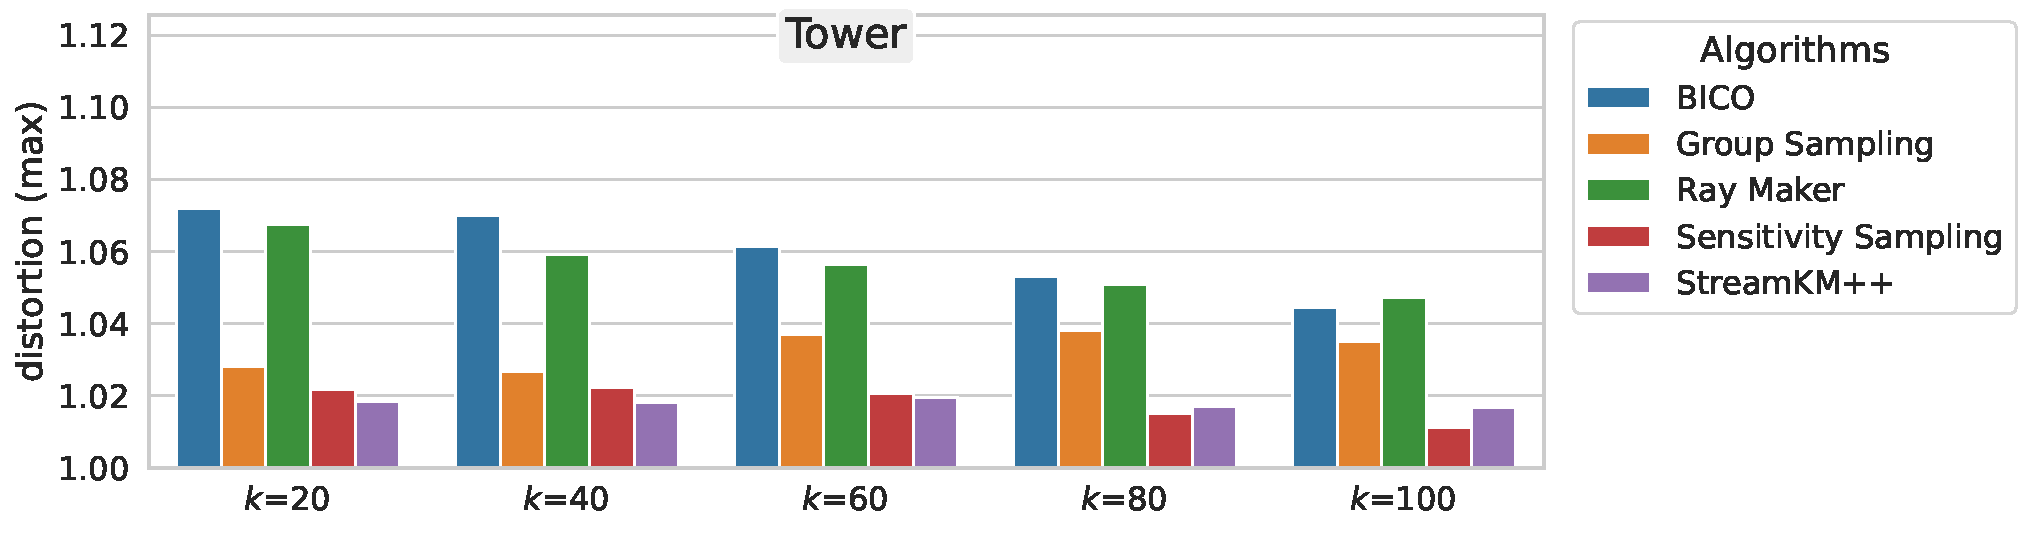
\includegraphics[width=.65\linewidth]{figures/distortions-Tower.pdf}
  \newline \newline
  \subfloat{
    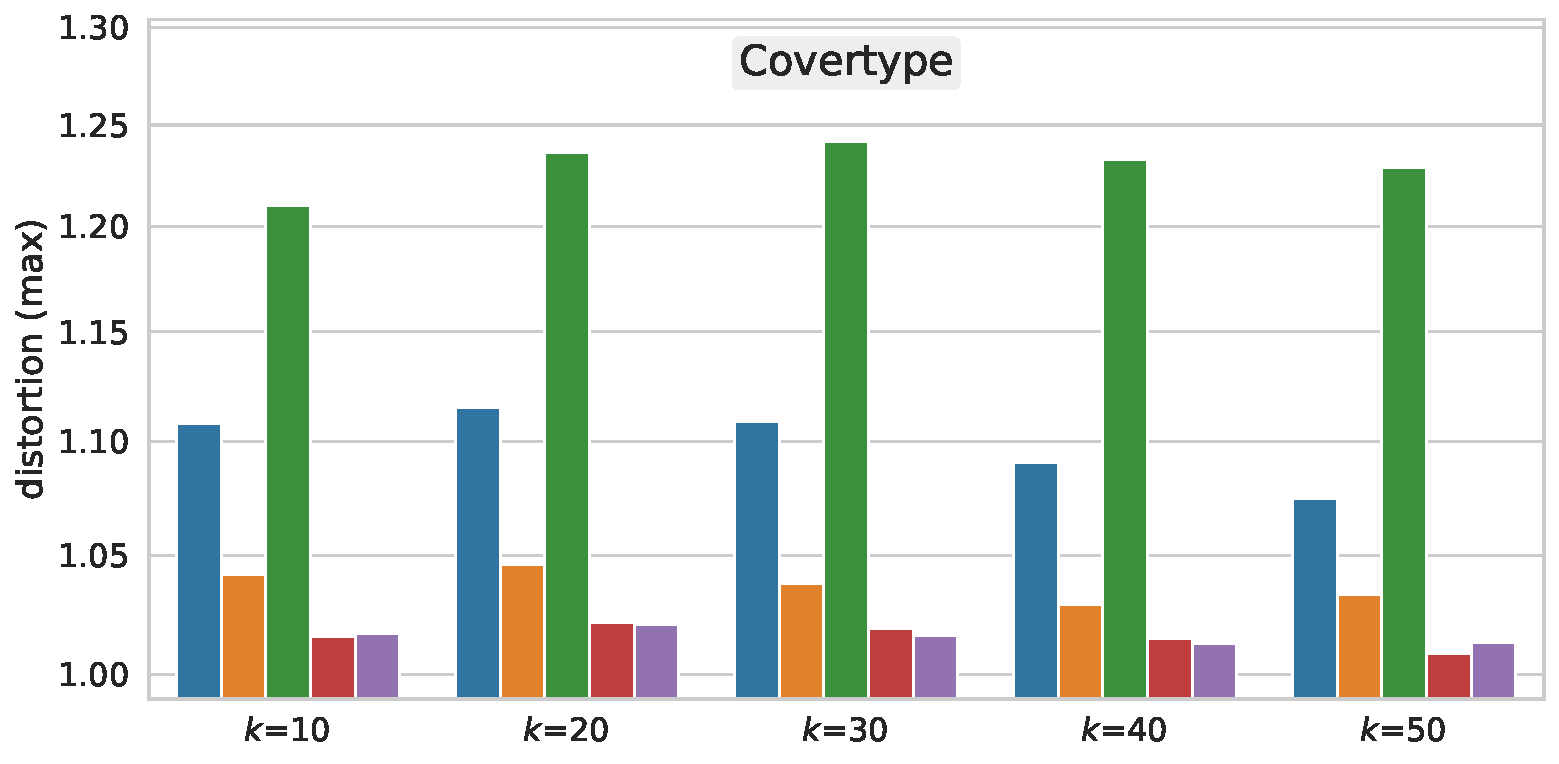
\includegraphics[width=0.5\textwidth]{figures/distortions-Covertype.pdf}
  }
  \subfloat{
    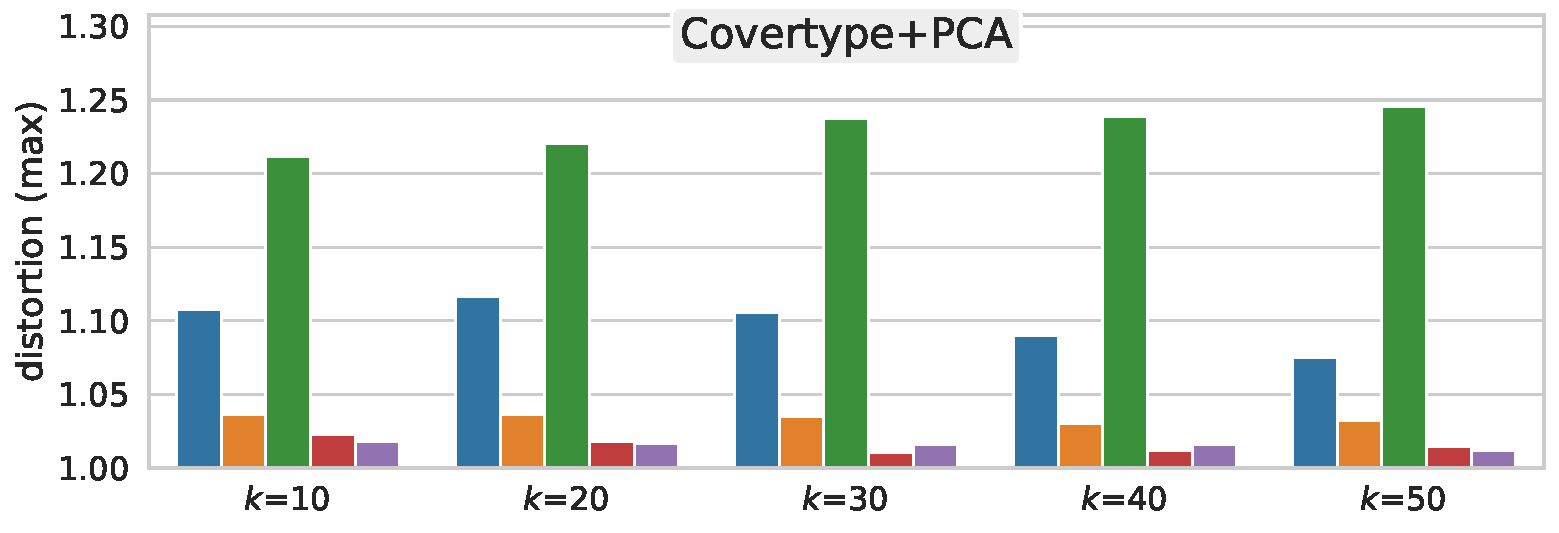
\includegraphics[width=.5\linewidth]{figures/distortions-Covertype+PCA.pdf}
  }
  \newline \newline
  \subfloat{
    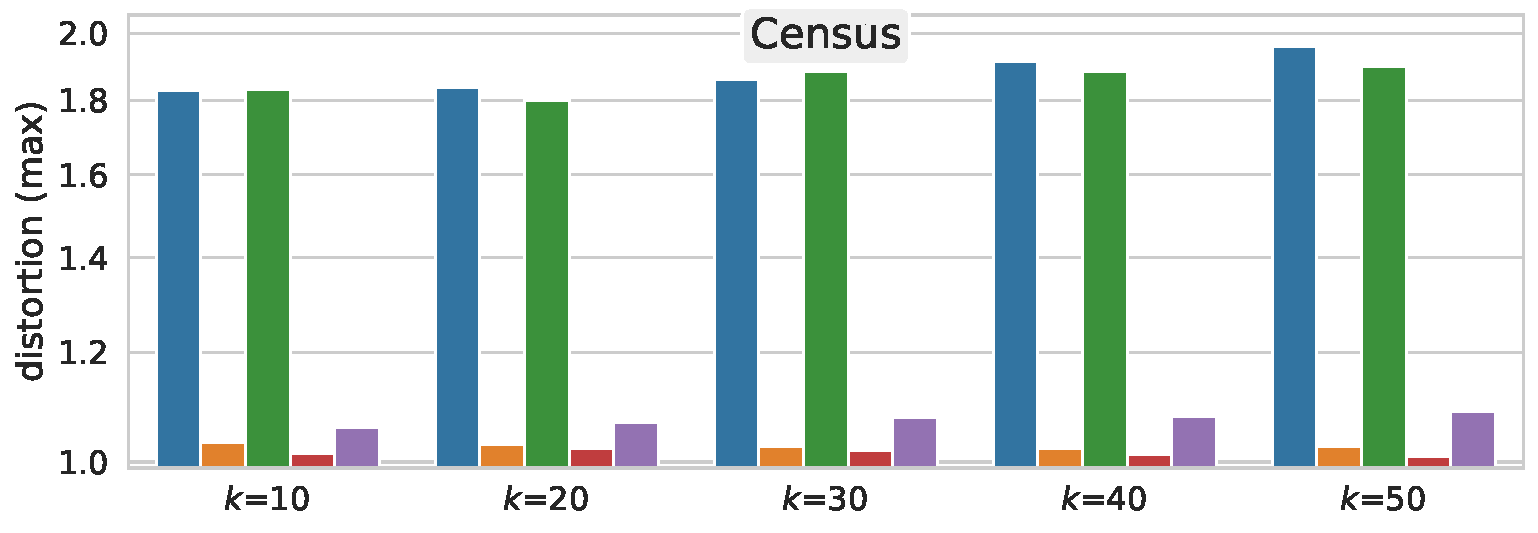
\includegraphics[width=0.5\textwidth]{figures/distortions-Census.pdf}
  }
  \subfloat{
    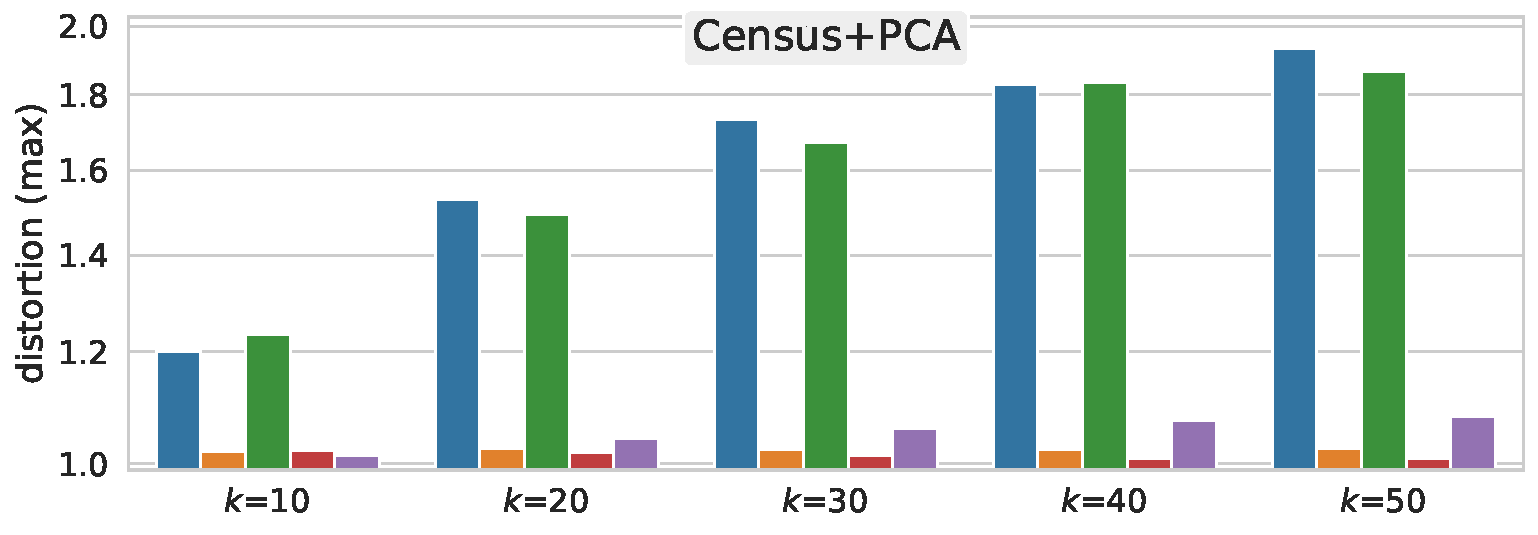
\includegraphics[width=.5\linewidth]{figures/distortions-Census+PCA.pdf}
  }
  \newline \newline
  \subfloat{
    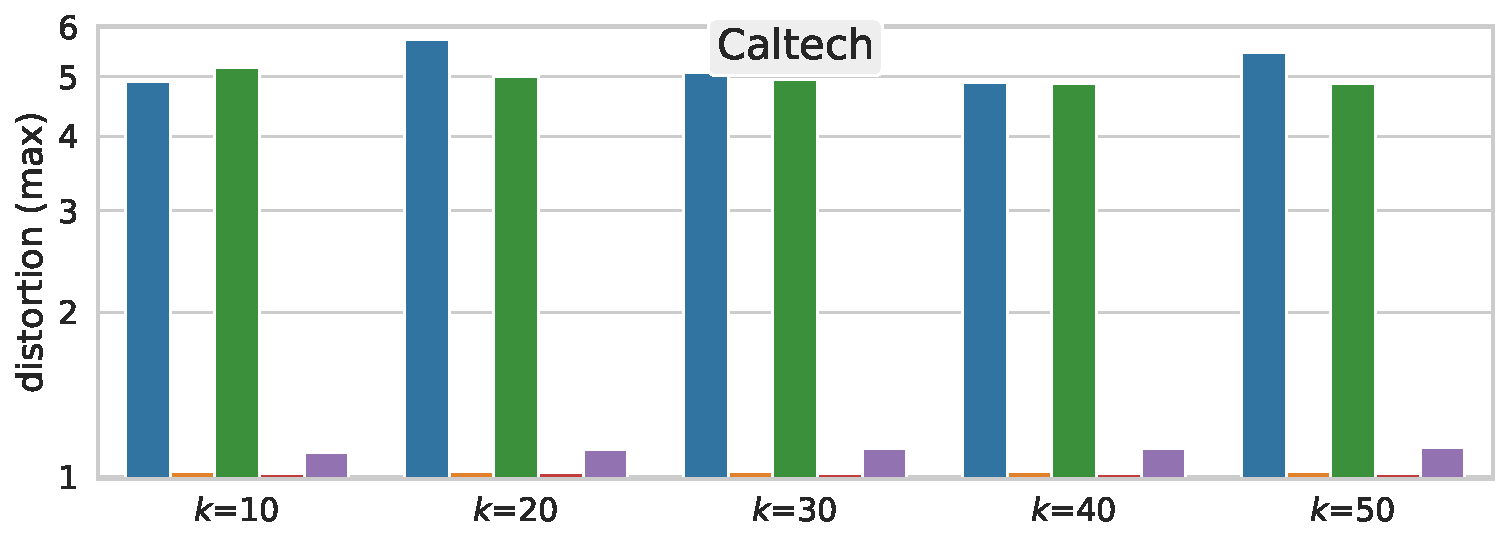
\includegraphics[width=0.5\textwidth]{figures/distortions-Caltech.pdf}
  }
  \subfloat{
    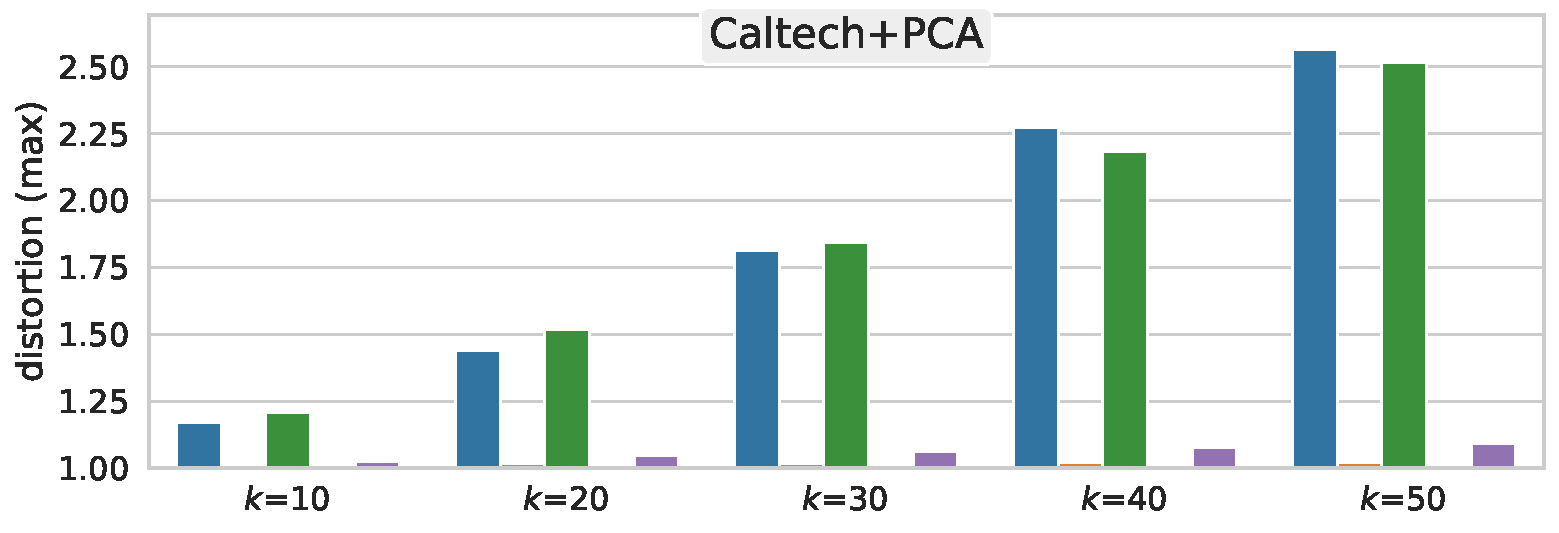
\includegraphics[width=.5\linewidth]{figures/distortions-Caltech+PCA.pdf}
  }
  \newline \newline
  \subfloat{
    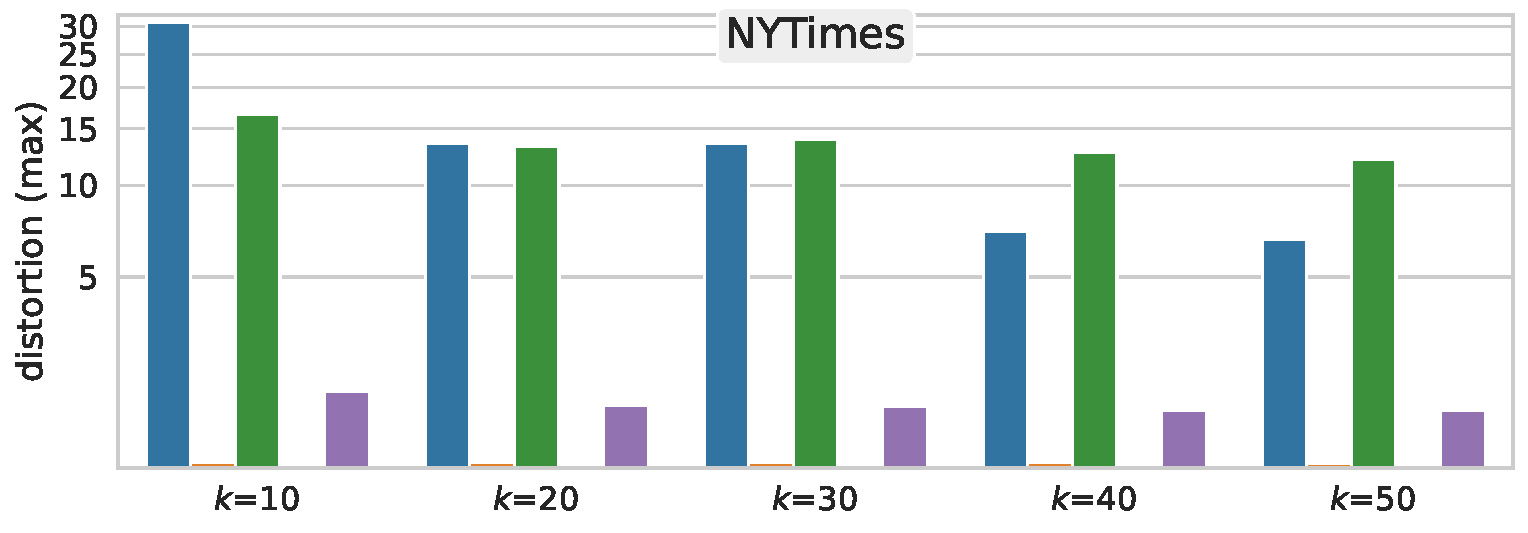
\includegraphics[width=0.5\textwidth]{figures/distortions-NYTimes.pdf}
  }
  \subfloat{
    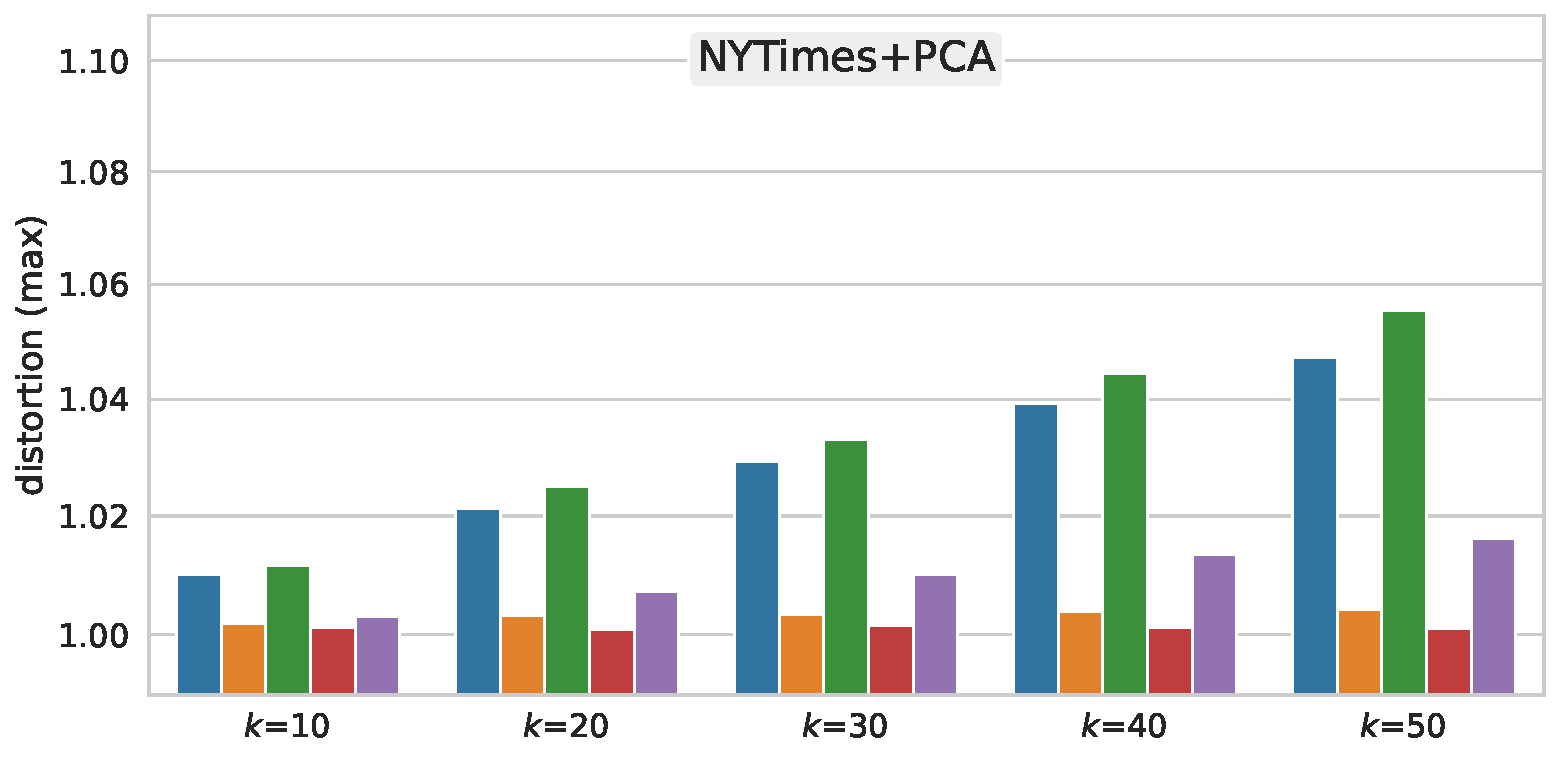
\includegraphics[width=.5\linewidth]{figures/distortions-NYTimes+PCA.pdf}
  }
  \newline \newline
  \subfloat{
    \\[1ex]
    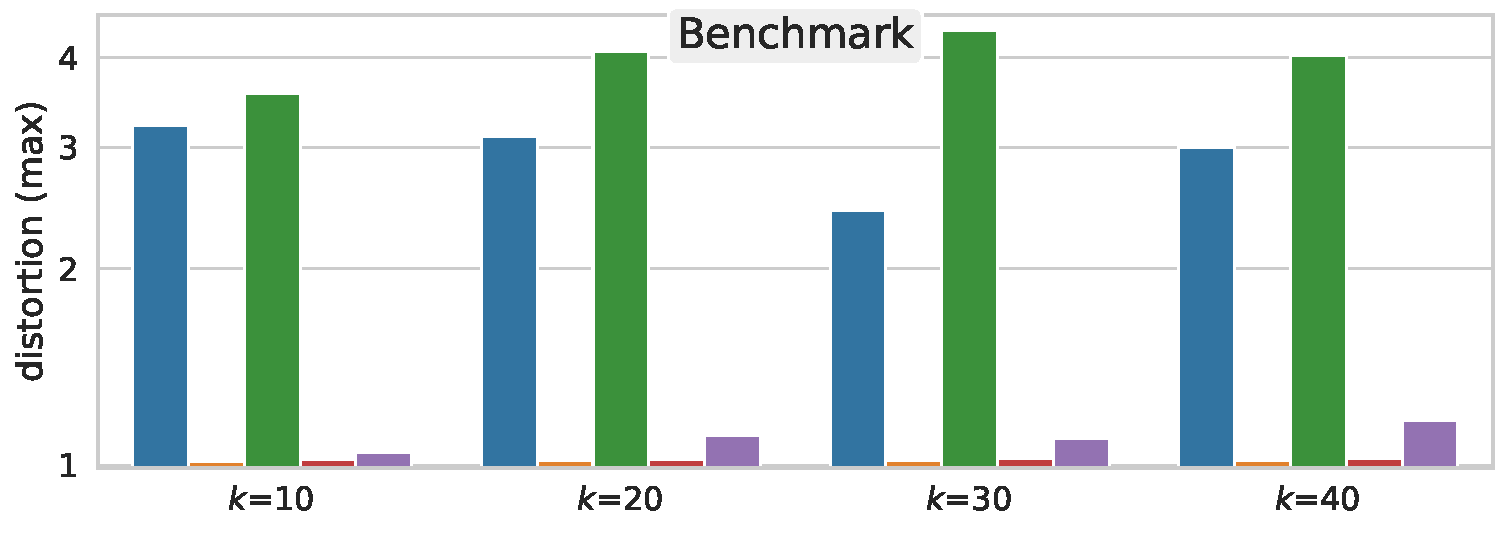
\includegraphics[width=0.5\textwidth]{figures/distortions-Benchmark.pdf}
  }
  \subfloat{
    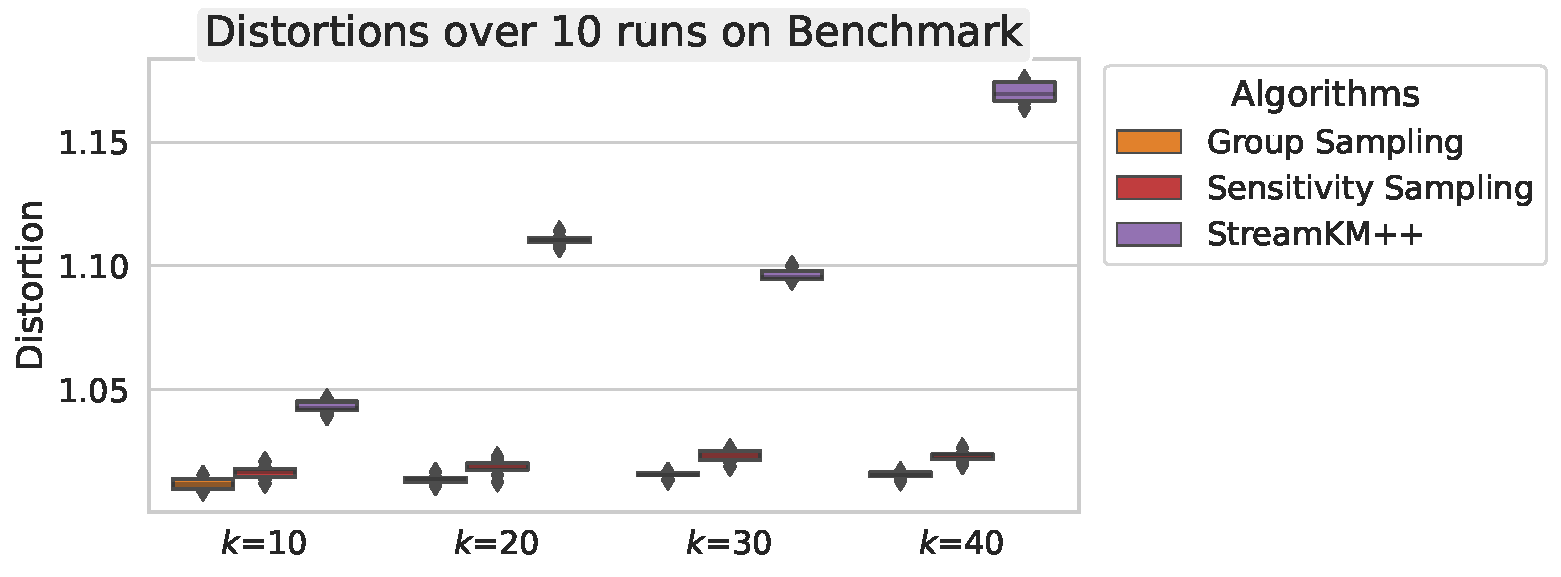
\includegraphics[width=.5\linewidth]{figures/boxplot-Benchmark-GS-SS-StreamKM.pdf}
  }
  
\end{figure*}

\begin{figure*}
  \caption{The real costs i.e. $\cost_A(\calS)$ of evaluated algorithms on 5 real-world datasets.}
  \label{fig:real-costs}
  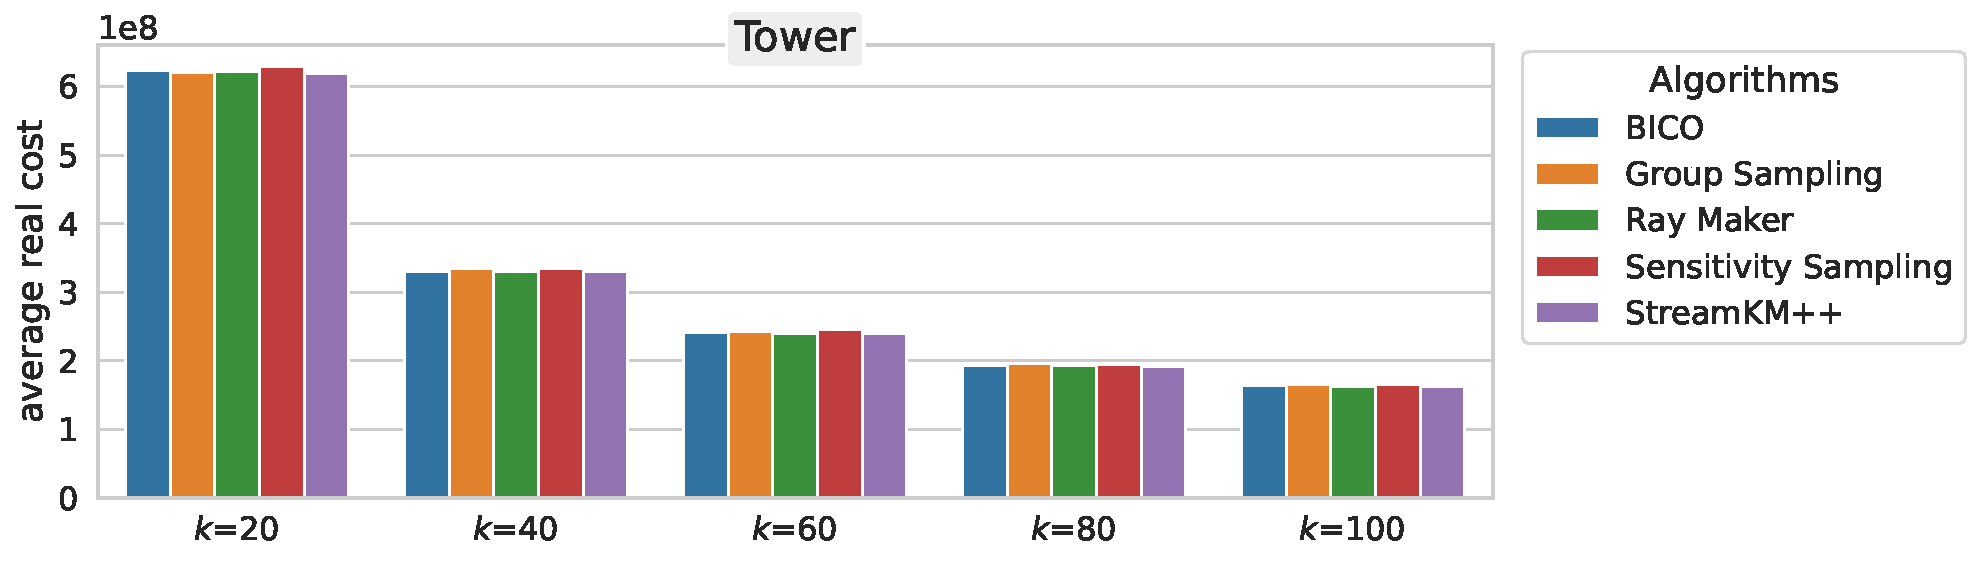
\includegraphics[width=.66\linewidth]{figures/real-costs-Tower.pdf}
  \newline
  \subfloat{
    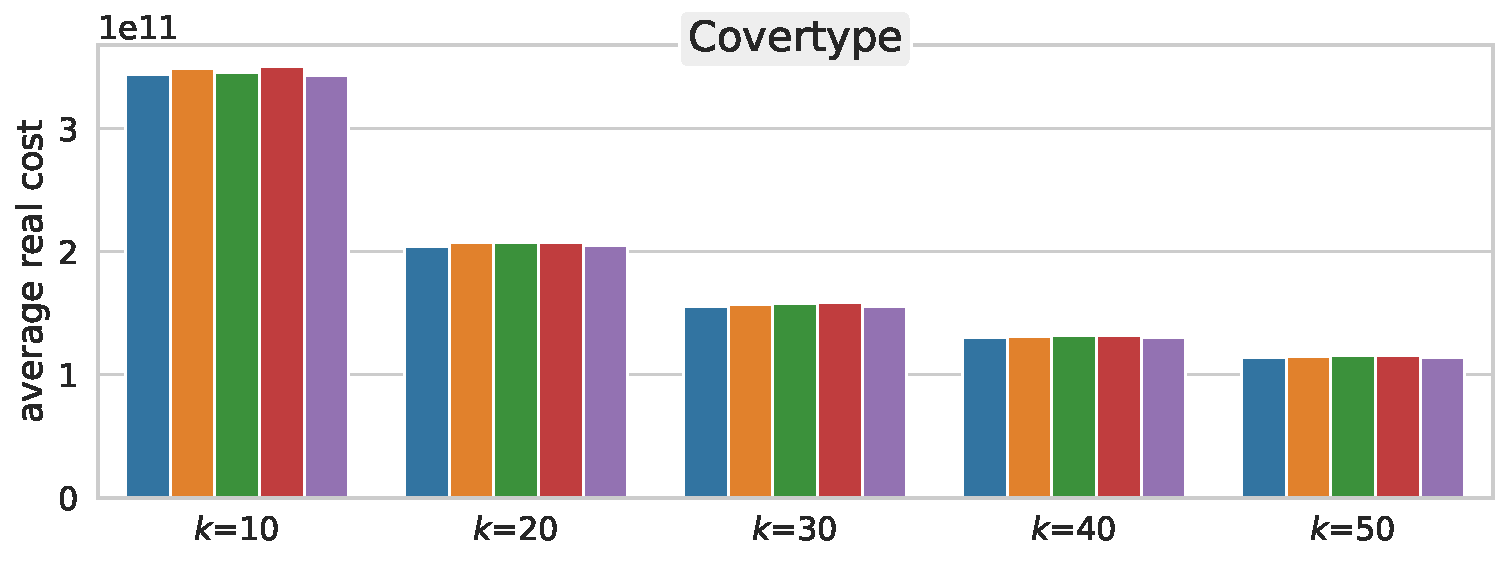
\includegraphics[width=0.5\textwidth]{figures/real-costs-Covertype.pdf}
  }
  \subfloat{
    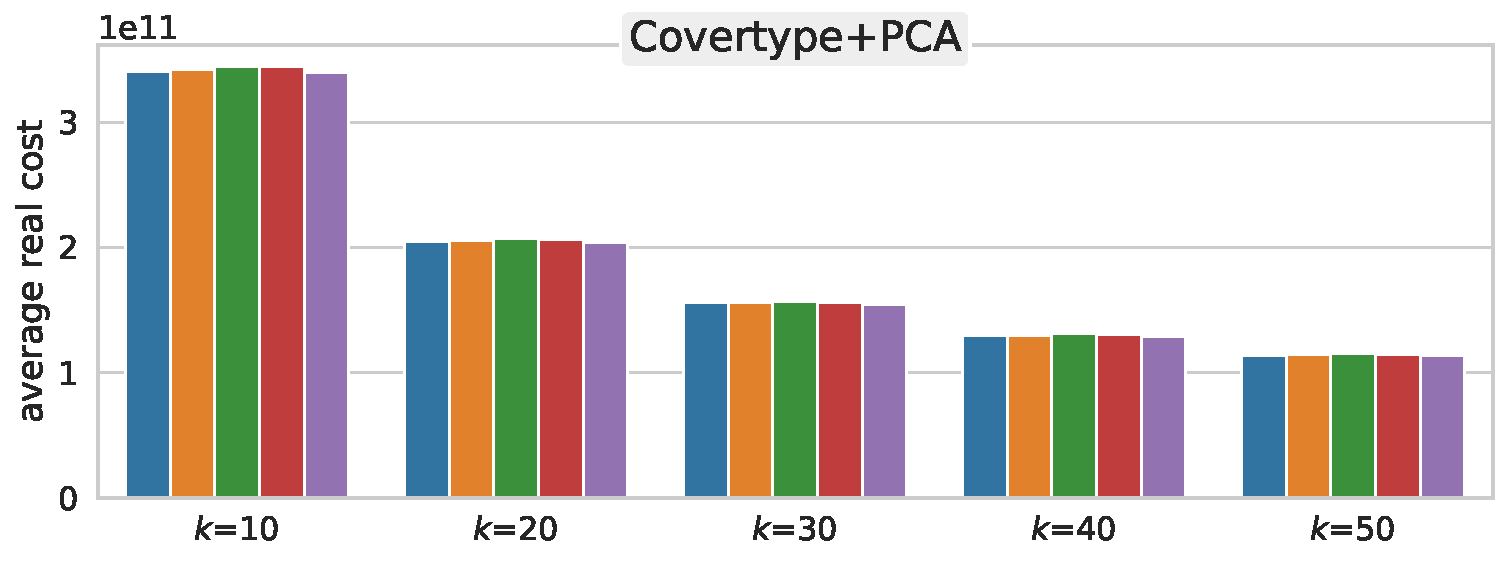
\includegraphics[width=.5\linewidth]{figures/real-costs-Covertype+PCA.pdf}
  }
  \newline
  \subfloat{
    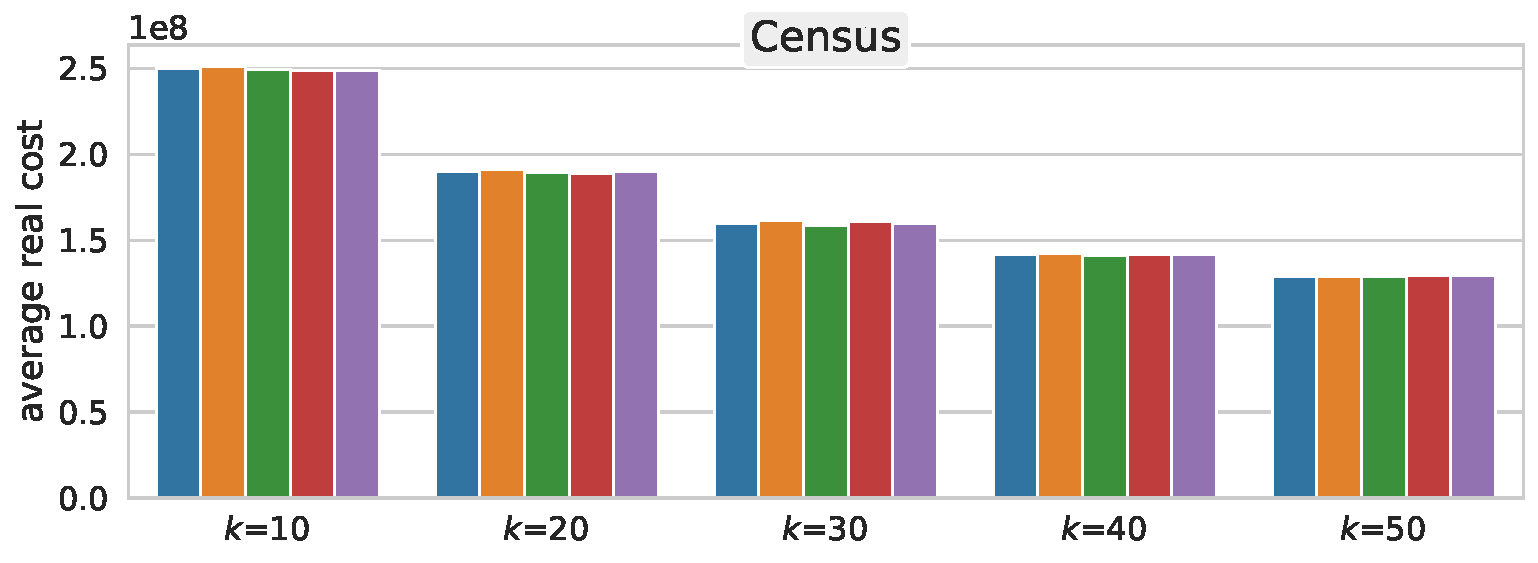
\includegraphics[width=0.5\textwidth]{figures/real-costs-Census.pdf}
  }
  \subfloat{
    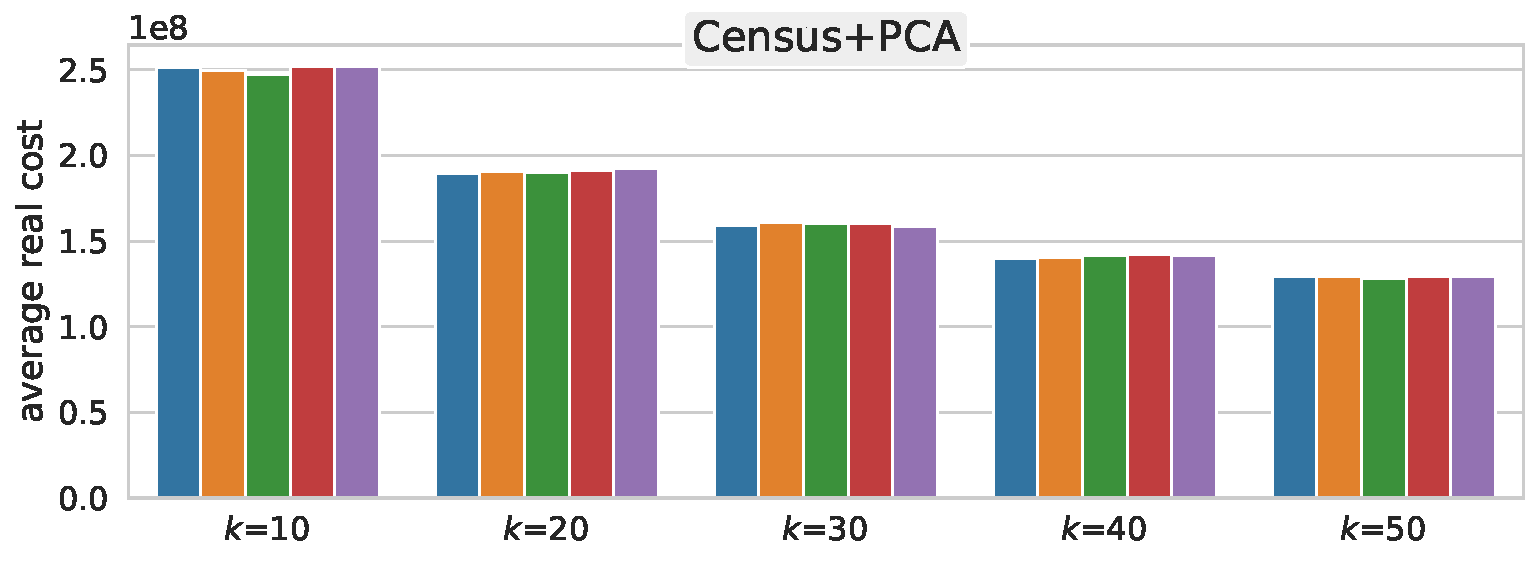
\includegraphics[width=.5\linewidth]{figures/real-costs-Census+PCA.pdf}
  }
  \newline
  \subfloat{
    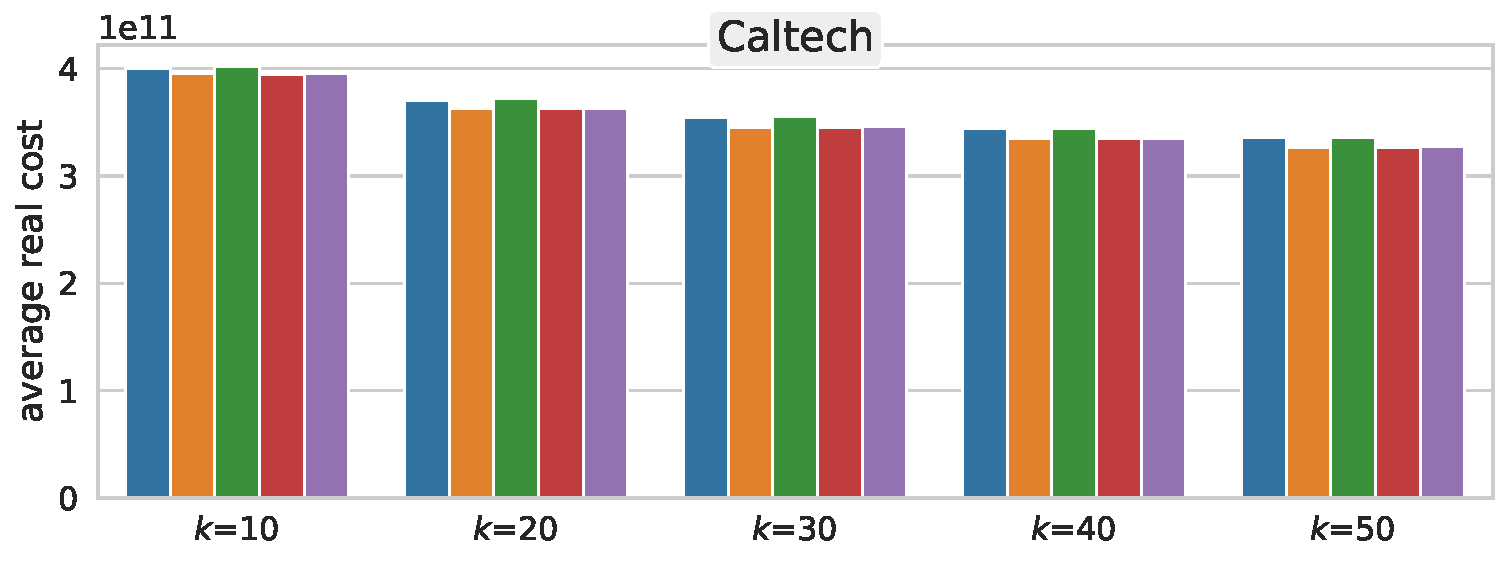
\includegraphics[width=0.5\textwidth]{figures/real-costs-Caltech.pdf}
  }
  \subfloat{
    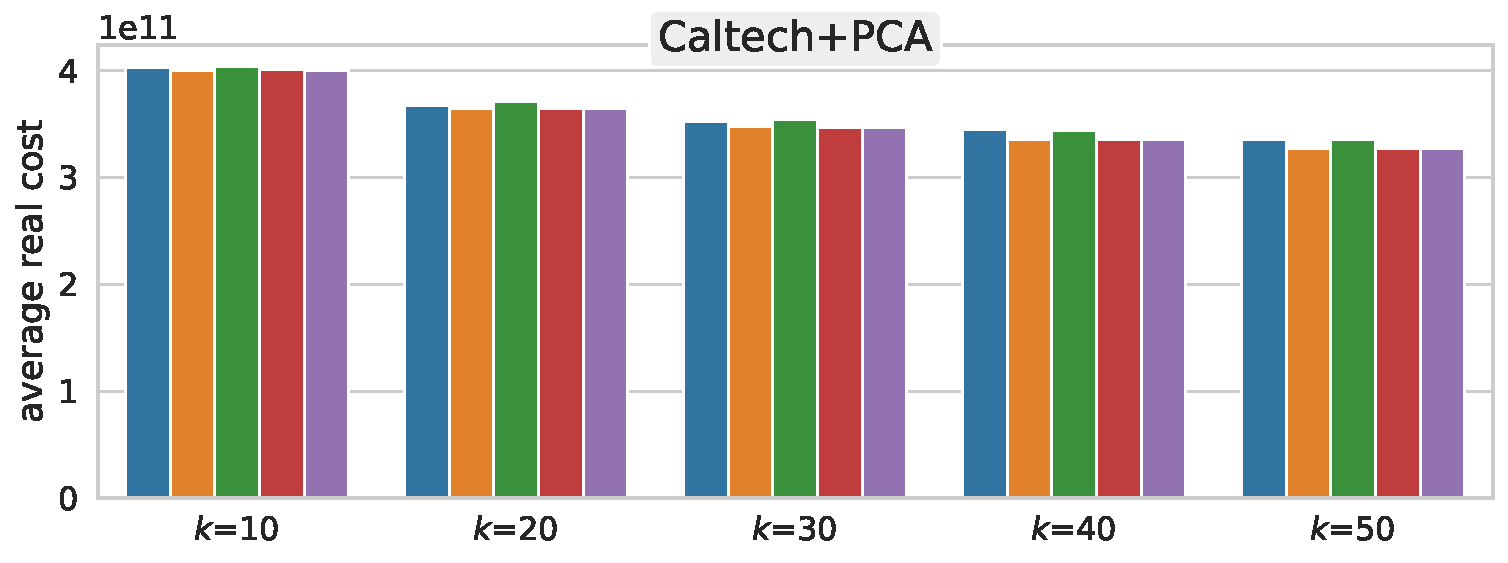
\includegraphics[width=.5\linewidth]{figures/real-costs-Caltech+PCA.pdf}
  }
  \newline
  \subfloat{
    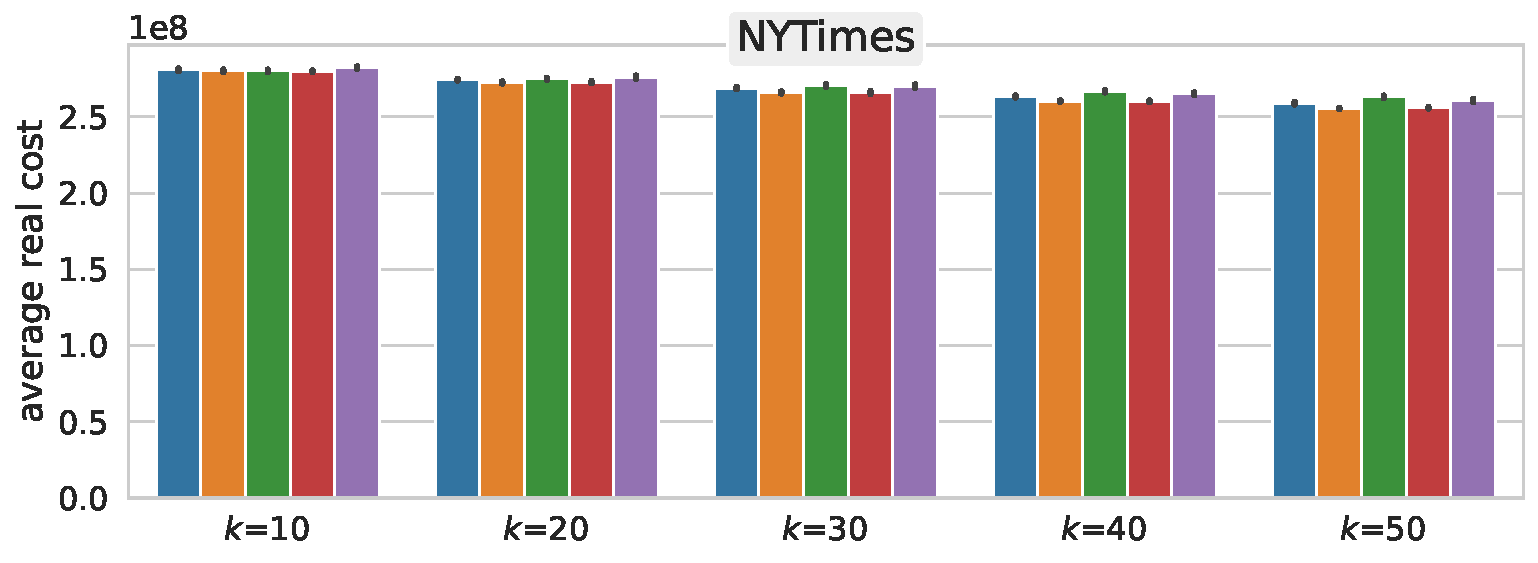
\includegraphics[width=0.5\textwidth]{figures/real-costs-NYTimes.pdf}
  }
  \subfloat{
    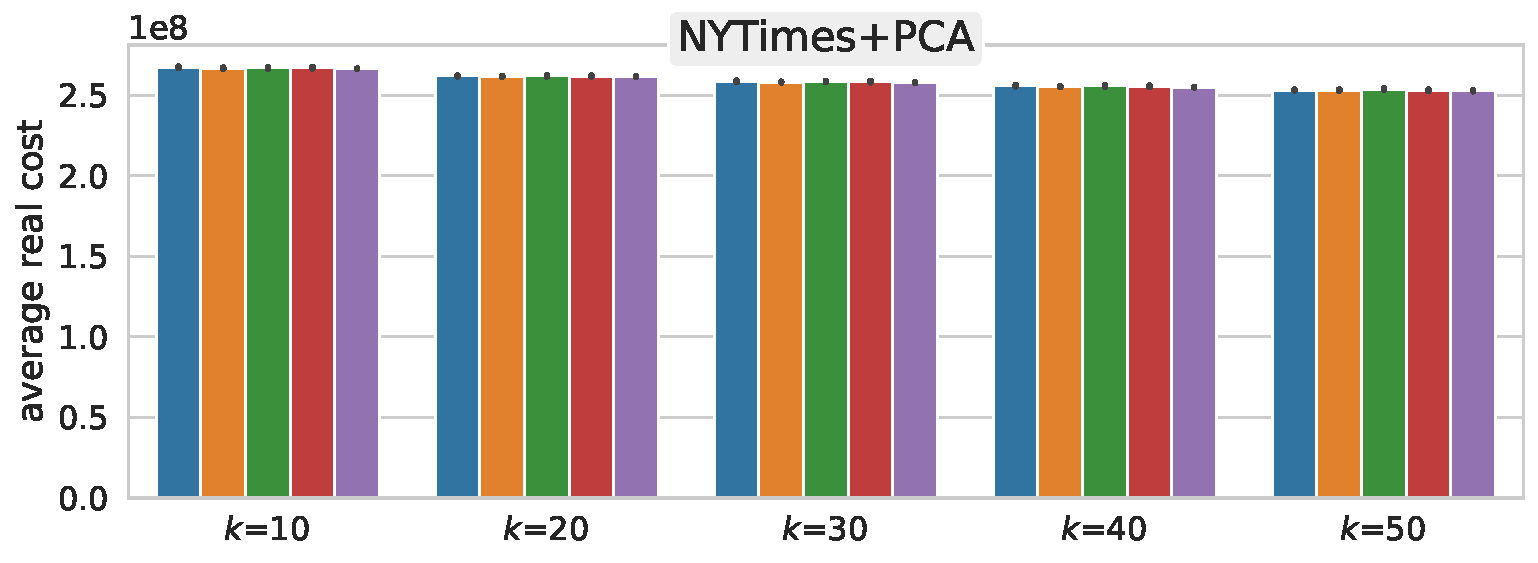
\includegraphics[width=.5\linewidth]{figures/real-costs-NYTimes+PCA.pdf}
  }
  \newline
  \subfloat{
    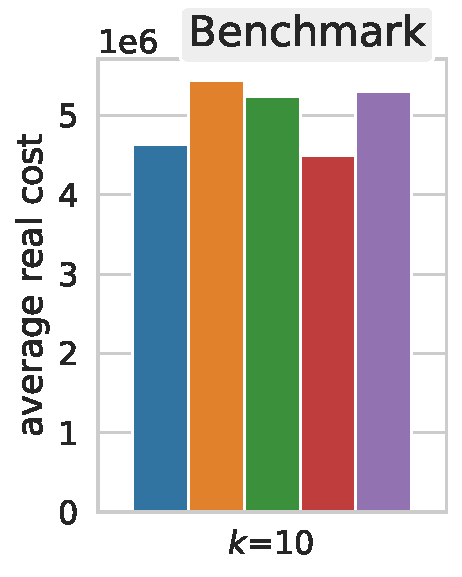
\includegraphics[width=0.15\textwidth]{figures/real-costs-Benchmark-k10.pdf}
    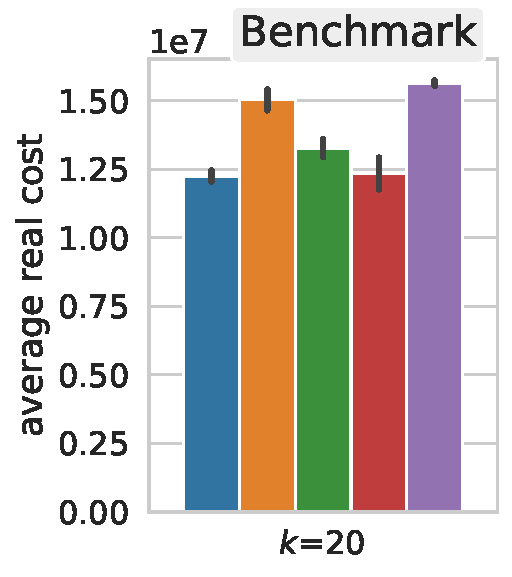
\includegraphics[width=0.165\textwidth]{figures/real-costs-Benchmark-k20.pdf}
    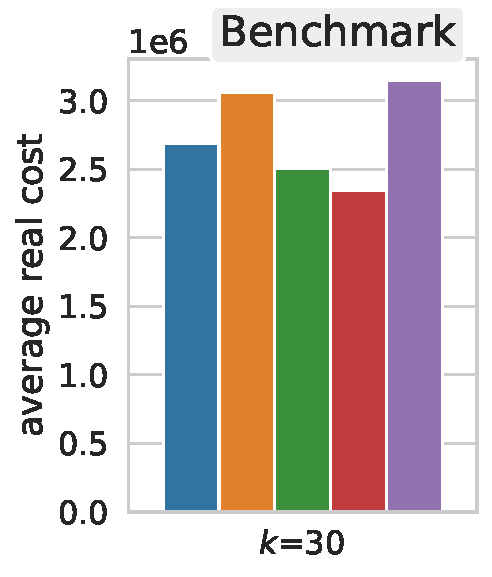
\includegraphics[width=0.16\textwidth]{figures/real-costs-Benchmark-k30.pdf}
    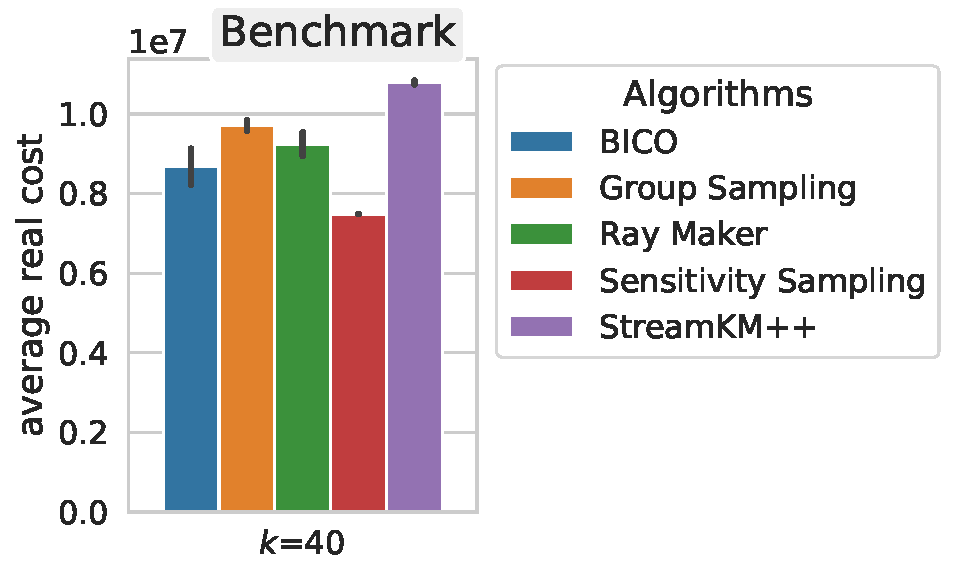
\includegraphics[width=0.31\textwidth]{figures/real-costs-Benchmark-k40.pdf}
  }
\end{figure*}





\begin{figure*}
  \caption{The coreset costs i.e. $\cost_\Omega(\calS)$ of evaluated algorithms on 5 real-world datasets.}
  \label{fig:coreset-costs}
  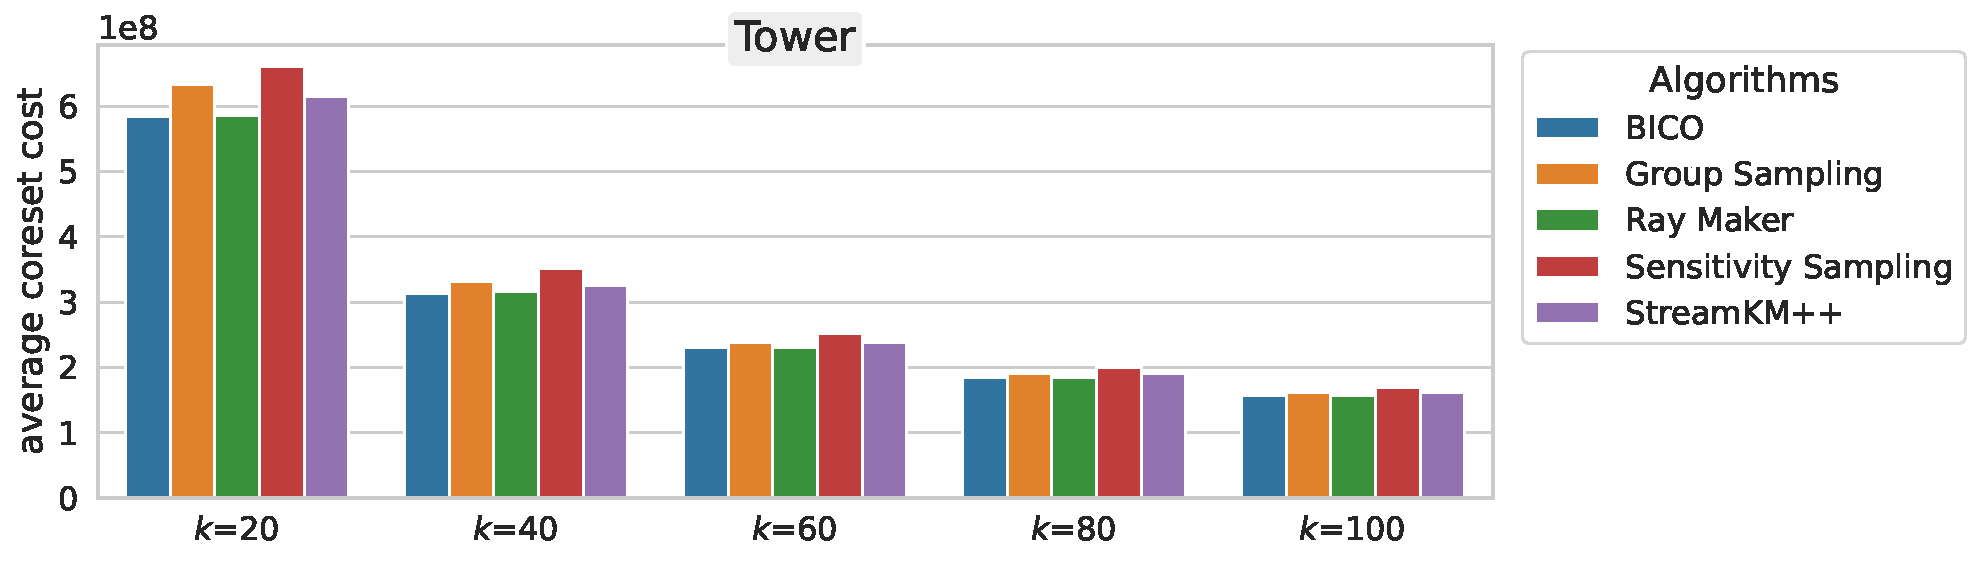
\includegraphics[width=.65\linewidth]{figures/coreset-costs-Tower.pdf}
  \newline
  \subfloat{
    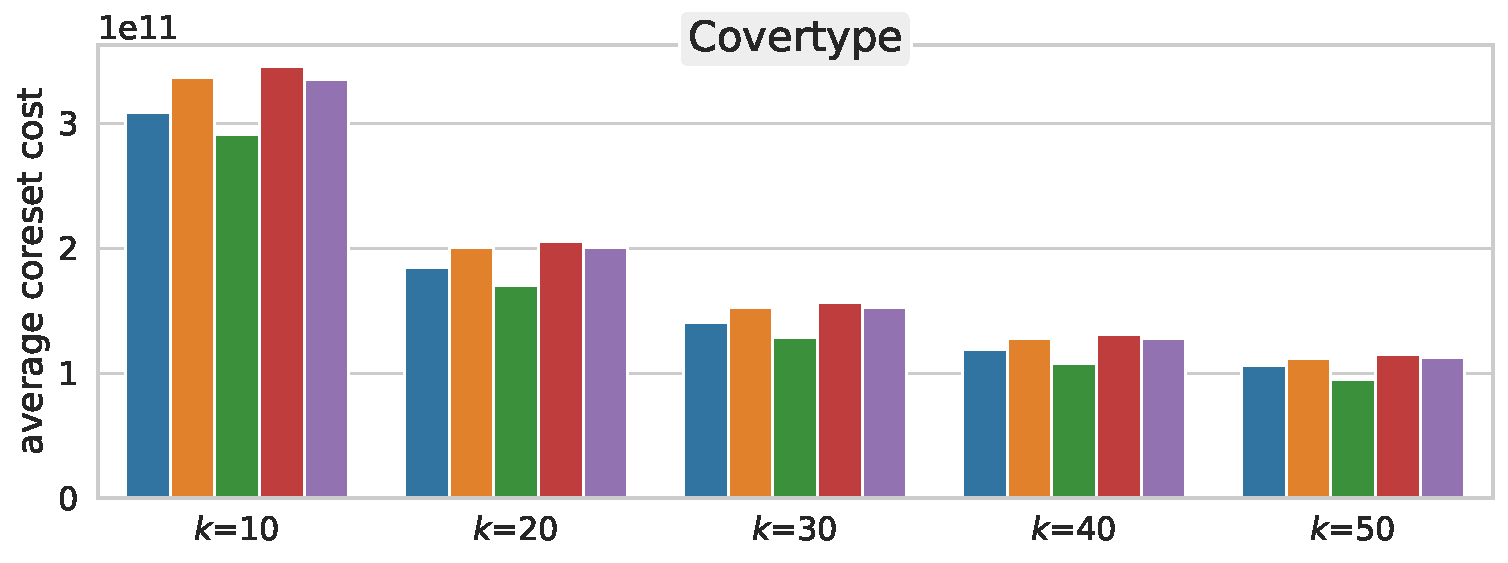
\includegraphics[width=0.5\textwidth]{figures/coreset-costs-Covertype.pdf}
  }
  \subfloat{
    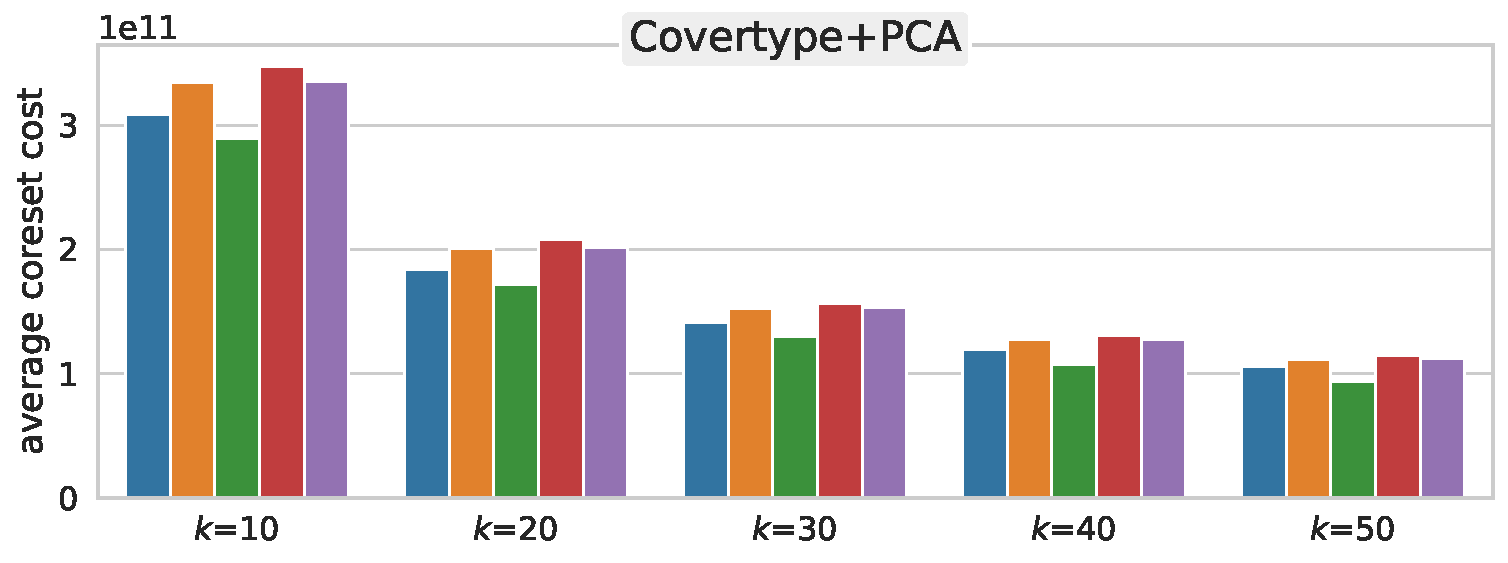
\includegraphics[width=.5\linewidth]{figures/coreset-costs-Covertype+PCA.pdf}
  }
  \newline
  \subfloat{
    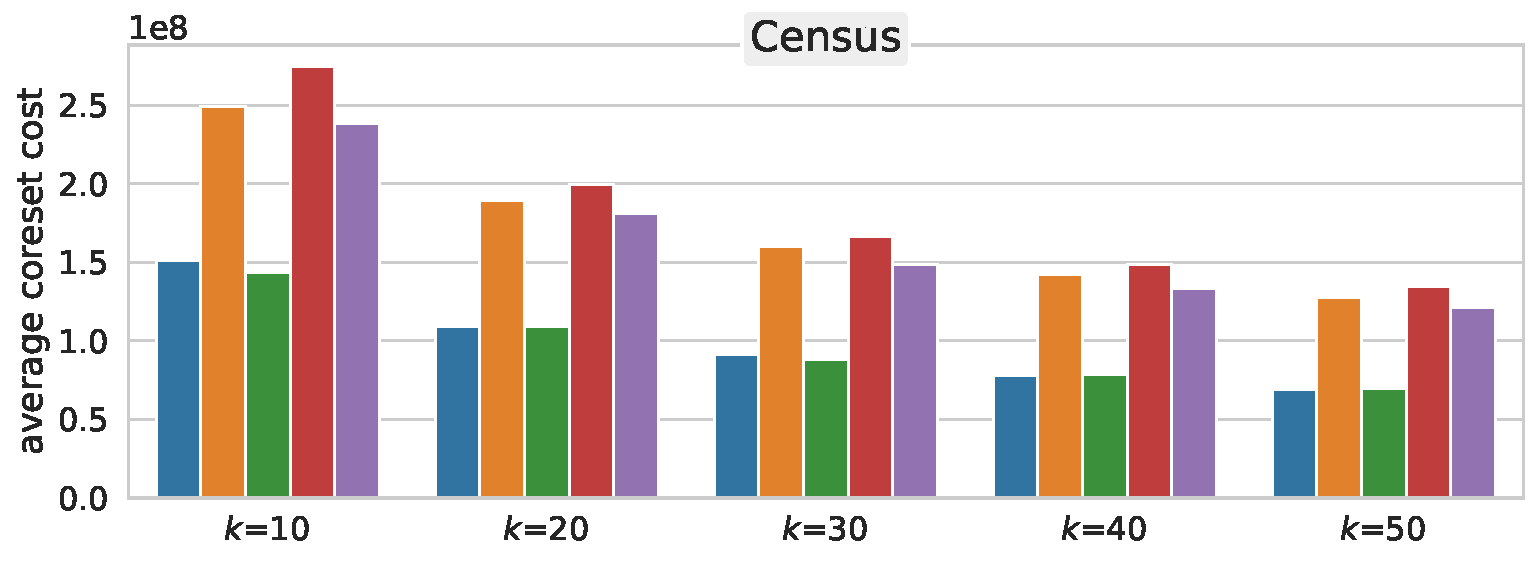
\includegraphics[width=0.5\textwidth]{figures/coreset-costs-Census.pdf}
  }
  \subfloat{
    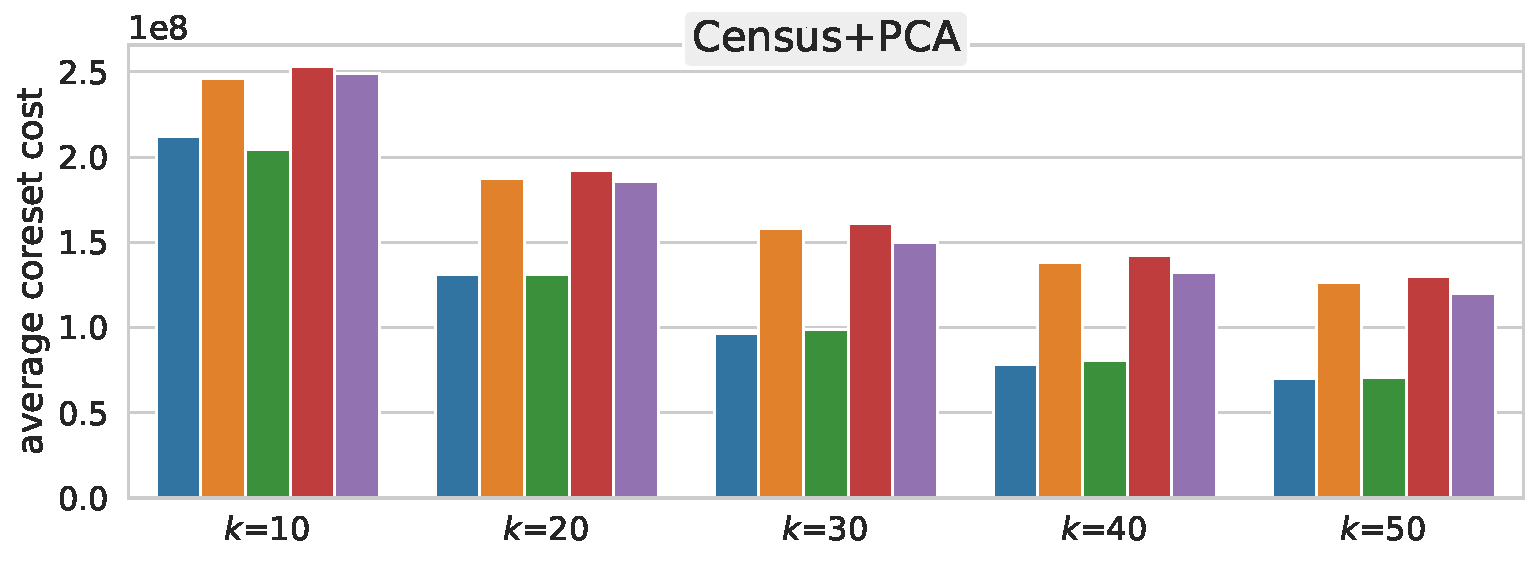
\includegraphics[width=.5\linewidth]{figures/coreset-costs-Census+PCA.pdf}
  }
  \newline
  \subfloat{
    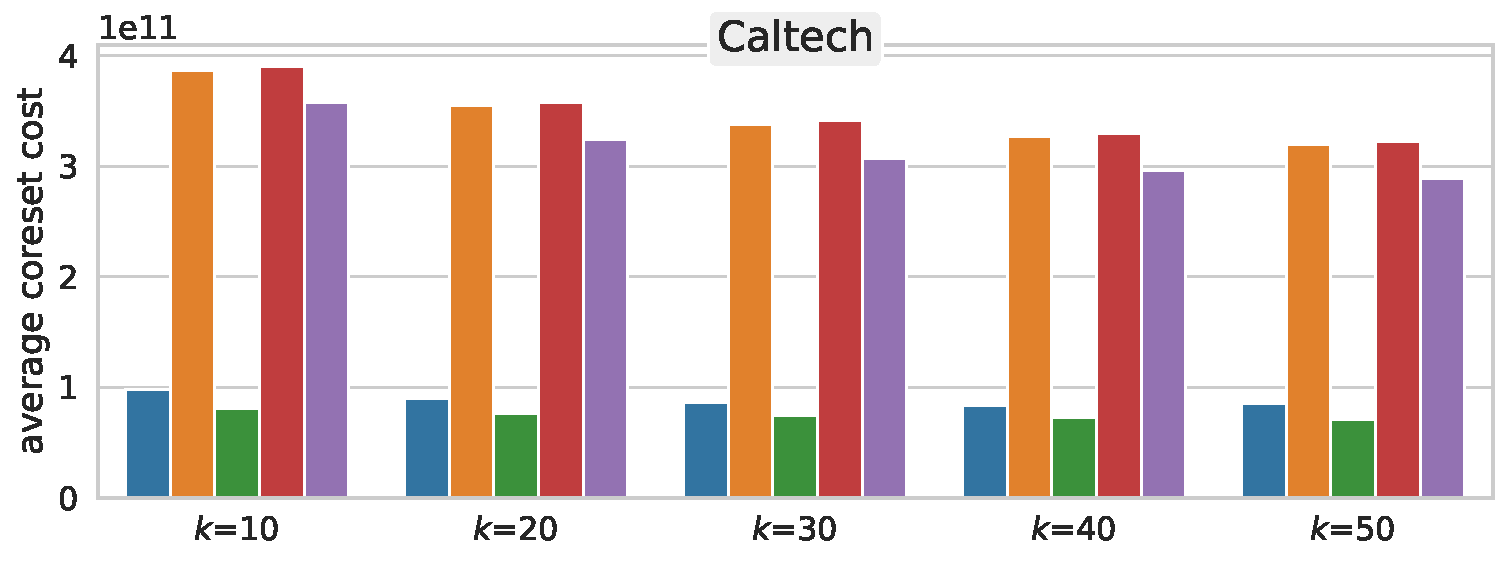
\includegraphics[width=0.5\textwidth]{figures/coreset-costs-Caltech.pdf}
  }
  \subfloat{
    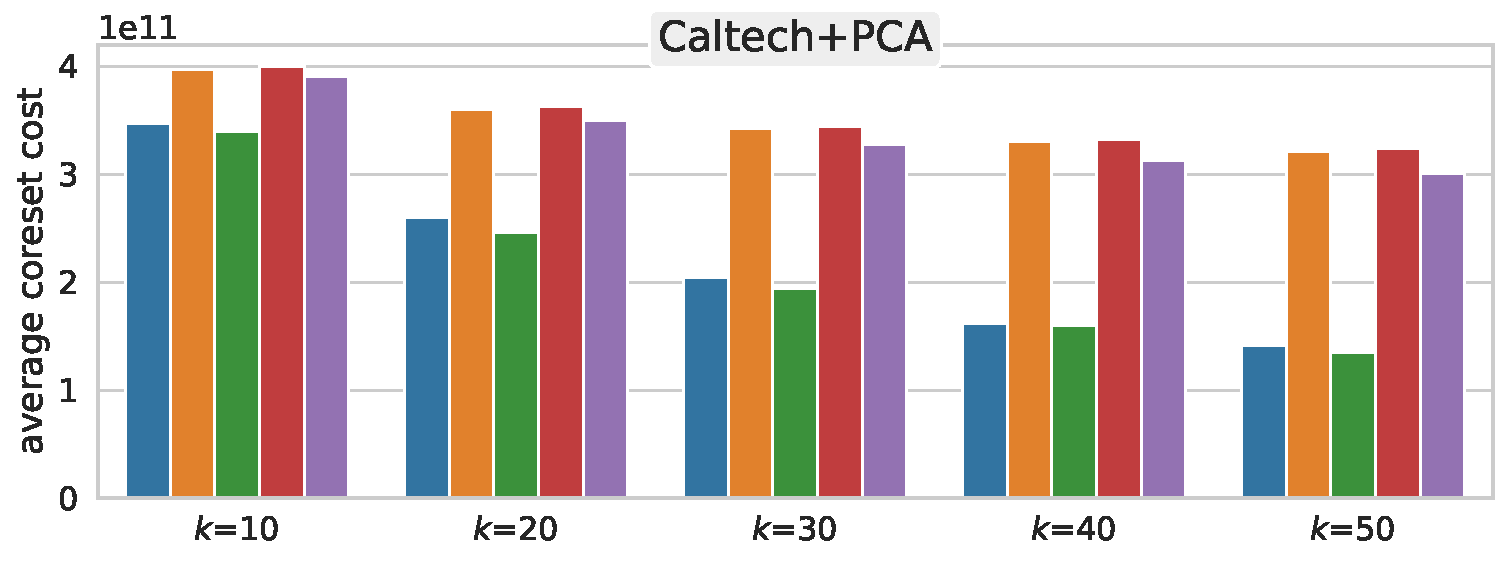
\includegraphics[width=.5\linewidth]{figures/coreset-costs-Caltech+PCA.pdf}
  }
  \newline
  \subfloat{
    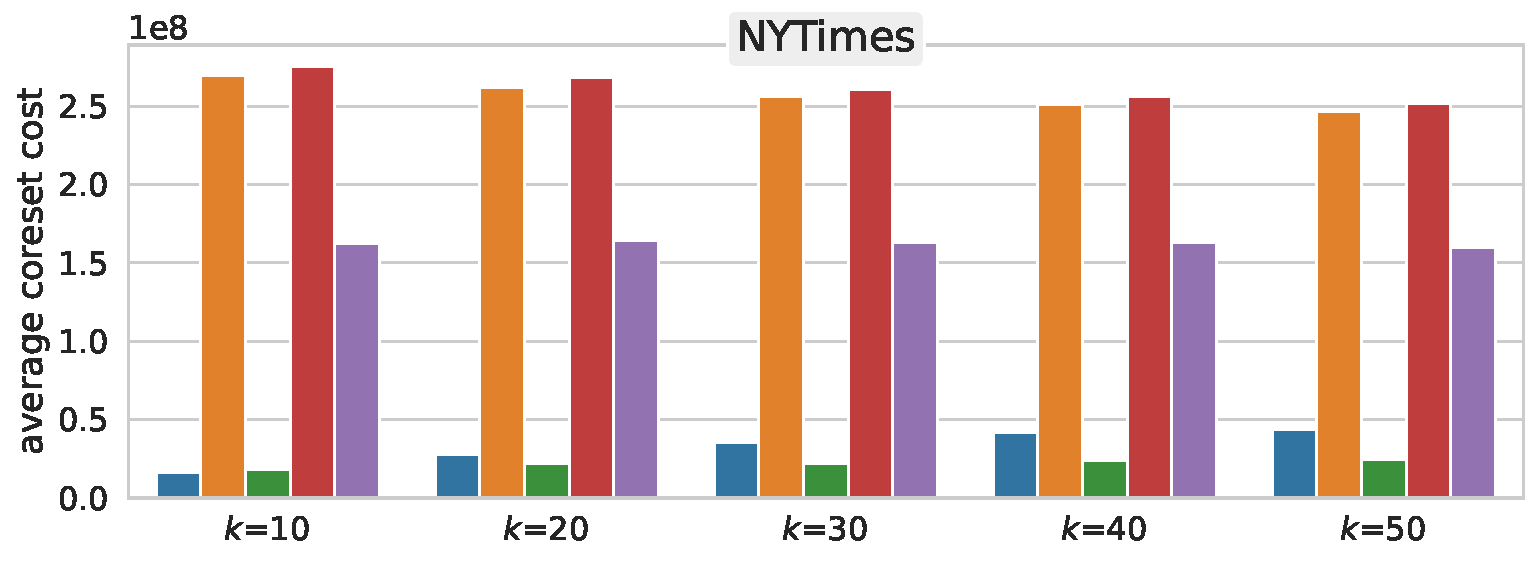
\includegraphics[width=0.5\textwidth]{figures/coreset-costs-NYTimes.pdf}
  }
  \subfloat{
    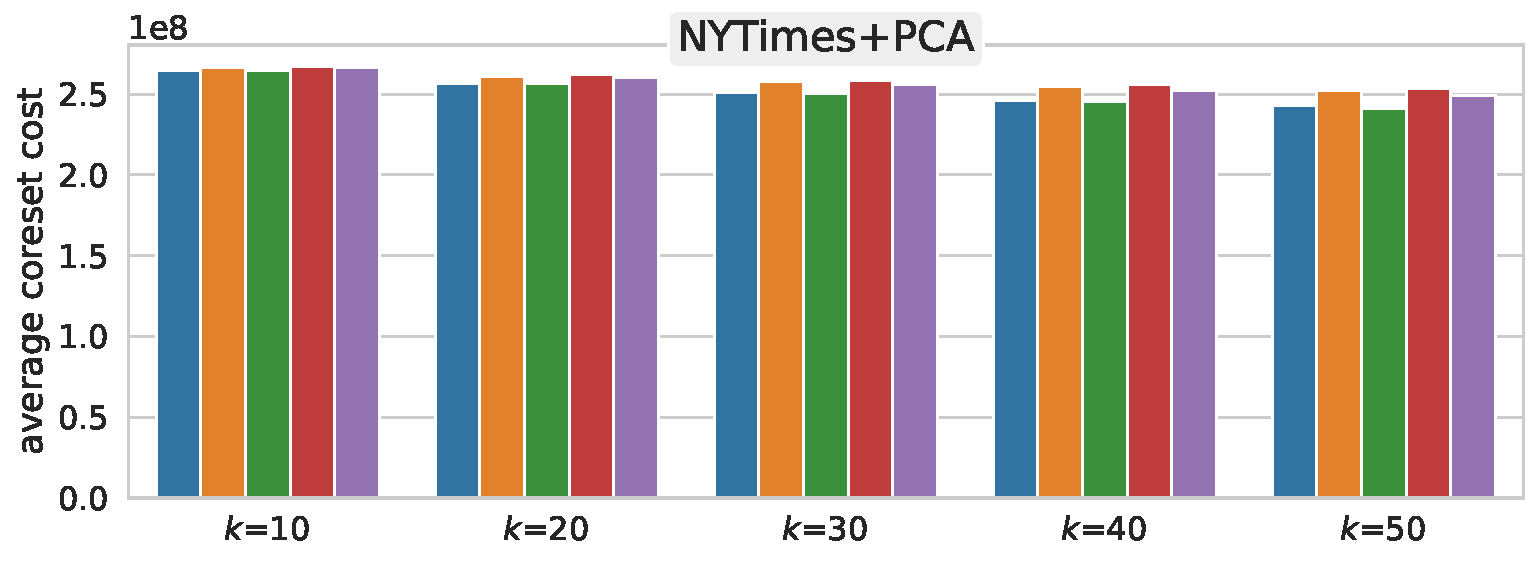
\includegraphics[width=.5\linewidth]{figures/coreset-costs-NYTimes+PCA.pdf}
  }
  \newline
%   \subfloat{
%     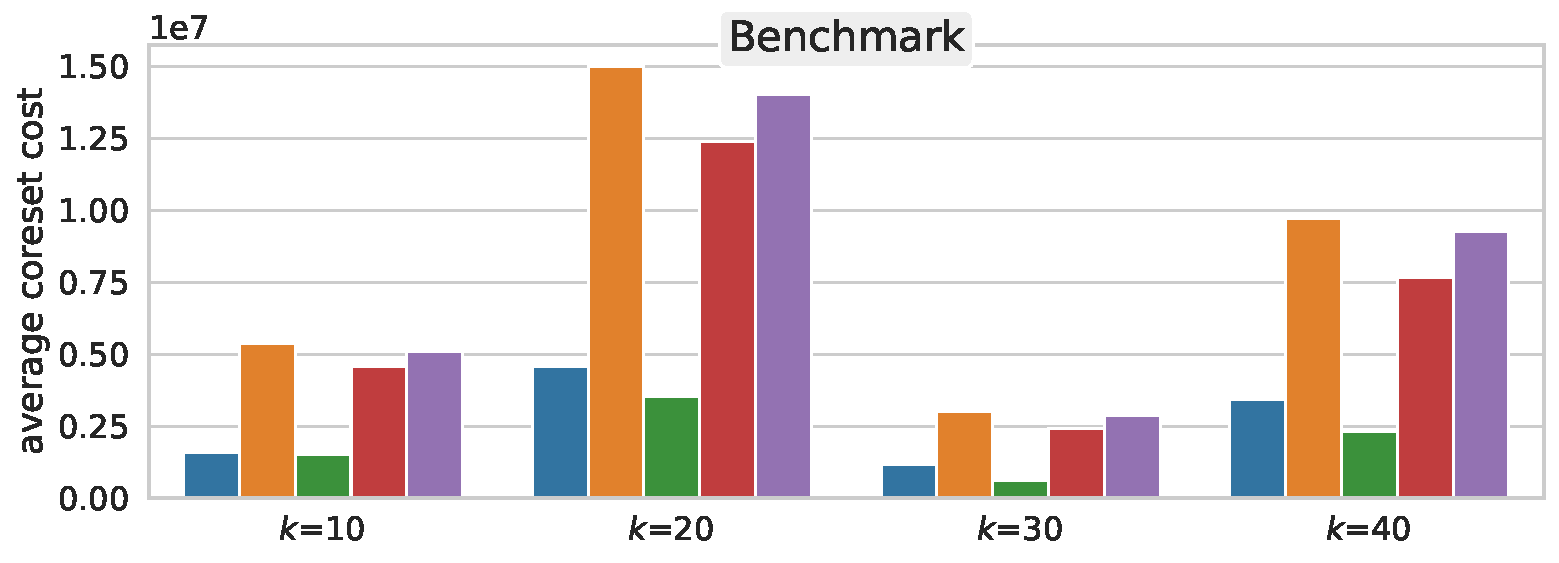
\includegraphics[width=0.5\textwidth]{figures/coreset-costs-Benchmark.pdf}
    
%   }
  \subfloat{
    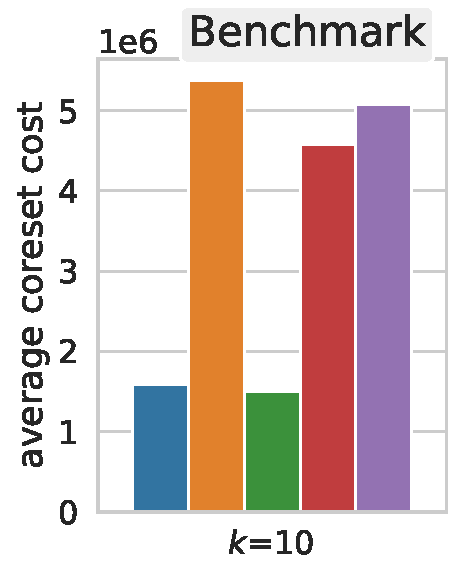
\includegraphics[width=0.15\textwidth]{figures/coreset-costs-Benchmark-k10.pdf}
    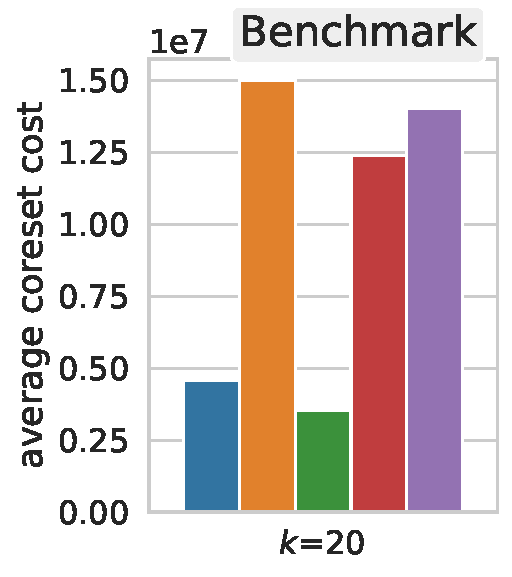
\includegraphics[width=0.165\textwidth]{figures/coreset-costs-Benchmark-k20.pdf}
    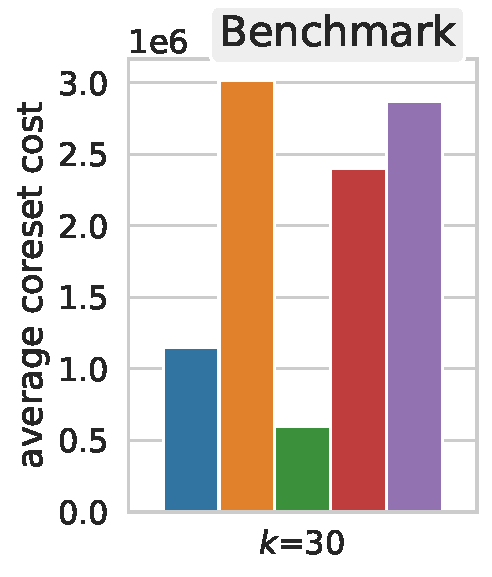
\includegraphics[width=0.16\textwidth]{figures/coreset-costs-Benchmark-k30.pdf}
    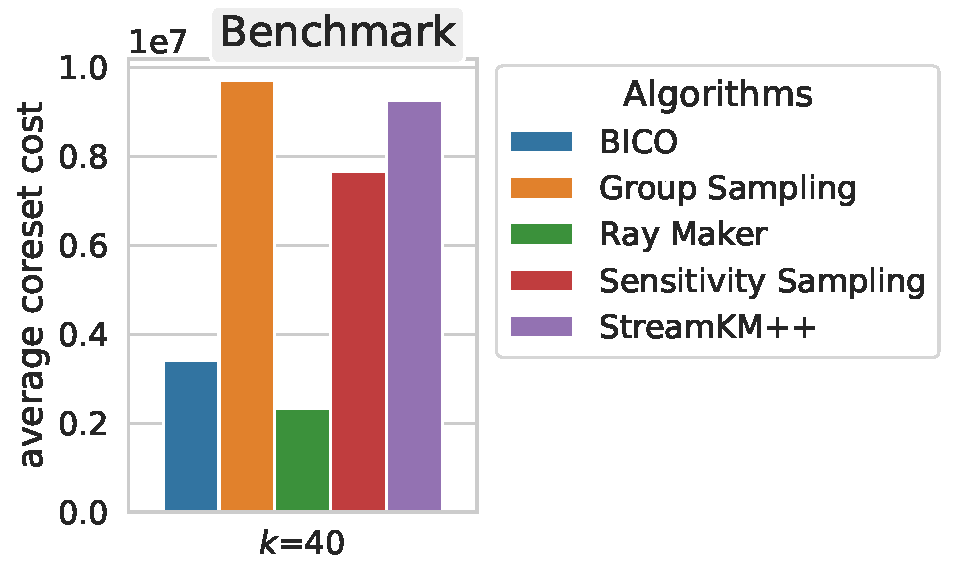
\includegraphics[width=0.31\textwidth]{figures/coreset-costs-Benchmark-k40.pdf}
  }
\end{figure*}






\subsection{Outcome of Experiments}
We summarized the distortions in \cref{fig:distortions}.
All five algorithms are matched on the \textit{Tower} dataset. The worst distortions across the algorithms are close to 1, and performance between the algorithms is negligible. The performance difference between sampling-based and movement-based methods become more pronounced as the number of dimensions increase. On \textit{Covertype} with its 54 features, Ray Maker performs the worst followed by BICO and Group Sampling while Sensitivity Sampling and StreamKM++ perform the best. Differences in performance are more noticeable on \textit{Census}, \textit{Caltech}, and \textit{NYTimes}  where methods based on importance sampling perform much better. Sensitivity Sampling and Group Sampling perform the best, StreamKM++ come in second while BICO and Ray Maker perform the worst across these data sets.
On the \textit{Benchmark}, Ray Maker is the worst while Sensitivty Sampling and Group Sampling are the best. StreamKM++ performs also very well compared to BICO.

Reducing noise with PCA helped boost the performance on real-world data sets with large number of dimensions. On \textit{Covertype}, PCA does not change the performance numbers by much. On \textit{Census} ($d=68$), the preprocessing step with PCA improves the performance of BICO and Ray Maker slightly for lower values of $k$. The distortions of BICO and Ray Maker are reduced markedly on \textit{Caltech} ($d=128$) after applying PCA. 


\subsection{Interpretation of Experimental Results}


\subsubsection*{Optimization versus Compression}
For some data sets, optimization is very close to compression. 
Clearly, this is the case for \textit{Tower}. The cost curve in ~\cref{fig:cost-curves-real-world-datasets} for this data set seem to support this claim as the elbow for \textit{Tower} bends the most which indicates that adding more centers help reduce the cost. For BICO, Ray Maker, and StreamKM++, there is a correlation between the steepness of the cost curve for a data set and the distortion of the generated coreset. For data sets where the curve is less steep, we observed higher distortions. The effect is more pronounced for the movement-based algorithms (BICO and Ray Maker) than for StreamKM++ which performs sampling. The other two sampling-based approaches (Group Sampling and Sensitivity Sampling) seem to be free from this behavior as they consistently generate high quality coresets irrespective of how the cost curve bends for a given data set.

\subsubsection*{Movement-based versus Sampling-based Approaches}
In general, movement-based constructions perform the worst in terms of coreset quality although all five algorithms are equally matched in terms of optimization. \cref{fig:real-costs} shows that the evaluated coreset constructions yield similar clusterings.
We observed that BICO and Ray Maker have the highest distortions across all datasets including on the benchmark instances. Among the sampling-based algorithms, Sensitive Sampling performs the best followed by Group Sampling and StreamKM++. Importance sampling seems to be superior than movement-based algorithms. On most data sets, StreamKM++ is the lowest performer among the three sampling-based methods. This can be attributed to the fact that the coreset produced by StreamKM++ consists entirely of $k$-means++ centers which mimic movement-based algorithms like BICO. Moreover, there is a movement-based component in the analysis of StreamKM++.





\subsubsection*{BICO versus StreamKM++}
Despite having the same worst case bounds, the quality of coresets produced by BICO and StreamKM++ differ significantly.
The theoretical analysis of the worst case bounds for BICO and StreamKM++ are derived from a movement-based construction. Both methods feature similar bounds as described in~\cref{sec:algorithms}. Surprisingly, the quality of the coresets produced by StreamKM++ is significantly better than what one would expect from the analysis. In terms of distortion StreamKM++ is significantly better than BICO across all datasets, and especially on high dimensionality data. This begs the question whether there exist a better theoretical analysis for StreamKM++. We leave this as an open problem for future research.



\subsubsection*{Impact of Noise Reduction}

\begin{figure}
  \caption{The cumulative propotion of explained variance by principal components on \textit{Caltech}, \textit{Covertype}, and \textit{Census}.}
  \label{fig:explained-variance-pca}
  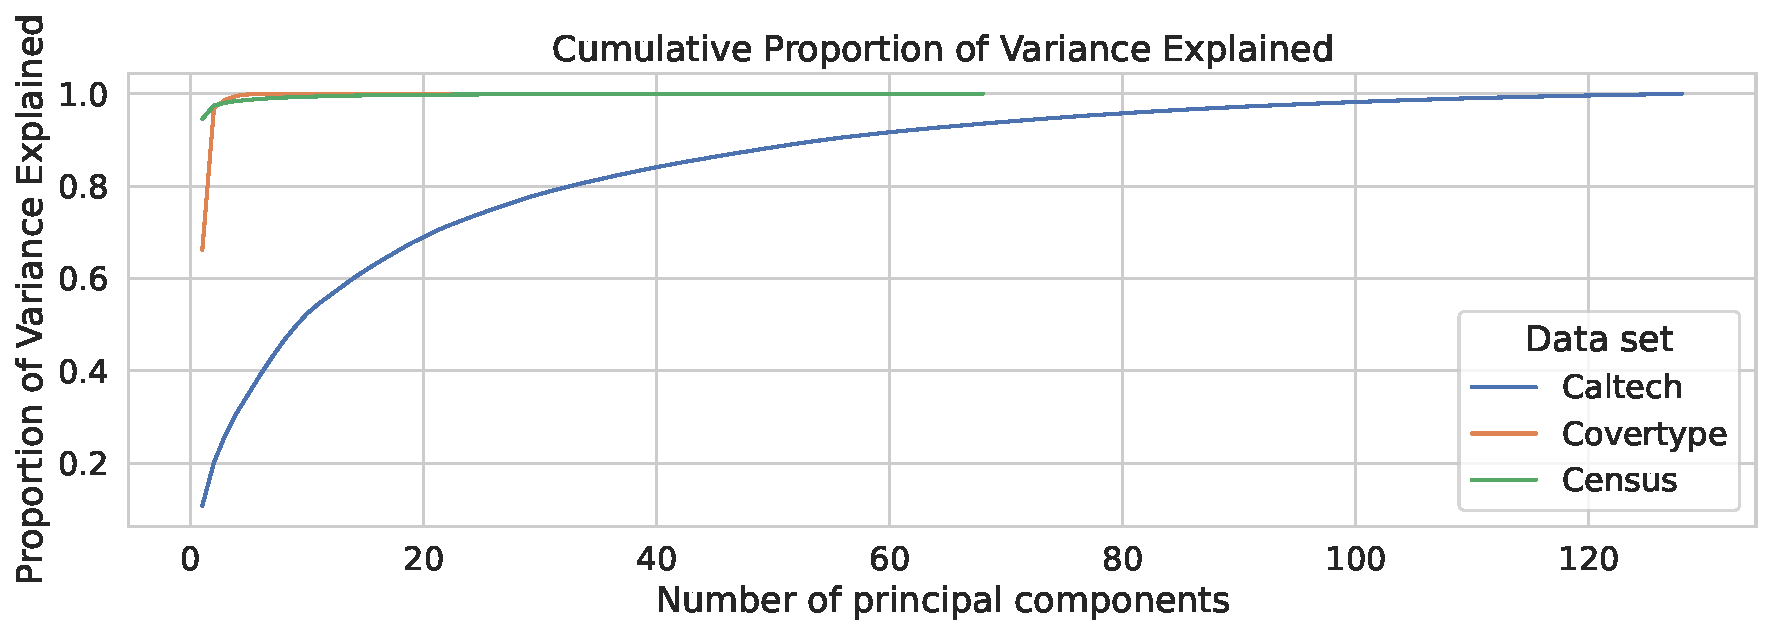
\includegraphics[width=1\linewidth]{figures/explained-variance-plot.pdf}
\end{figure}

On almost all our data sets, the performance improves when input data is preprocessed with PCA, especially for the movement-based algorithms. Empirically, the more noise is removed (i.e., small $k$ value), the lower the distortion. Notice that $k$ is the number of principal components that the input data is projected on to. The rest of the low variance components are treated as noise and removed. Method utilizing sampling (Group Sampling, Sensitivity Sampling and StreamKM++) are less effected by the preprocessing step. On \textit{Covertype}, PCA does not change the distortions by much because almost all the variance in the data is explained by the first five principal components (see~\cref{fig:explained-variance-pca}). As the smallest number of centers $k$ is $10$, the input data is simply being rotated. Similar explanation applies to the \textit{Census} data set. On our two high-dimensionality data sets \textit{Caltech} and \textit{NYTimes}, the quality of the coresets by BICO and Ray Maker improves greatly because the noise removal is more aggressive. Even if the quality is much better for movement-based coreset constructions due to PCA transformation, importance sampling methods are still superior when it comes to the quality of the compression. 

